\documentclass[a4paper,11pt]{article}
\usepackage{fullpage}
\usepackage{hyperref}
\usepackage{amsmath}
\usepackage{amssymb}
\usepackage{amsthm}
\usepackage{fancybox}
\usepackage{graphicx}
\usepackage{caption}
\usepackage{subcaption}
\usepackage{float}
\usepackage{natbib}
\bibliographystyle{abbrv}

\newtheorem{corollary}{Corollary}
\newtheorem{theorem}{Theorem}
\newtheorem{lemma}{Lemma}
\newtheorem{definition}{Definition}
\newtheorem{proposition}[theorem]{Proposition}
\newtheorem{warning}[theorem]{Warning}
\newcommand{\CAT}{\textrm{CAT}}
\newcommand{\BHV}{\textrm{BHV}}
\newcommand{\aC}{\mathcal{C}}
\newcommand{\aD}{\mathcal{D}}
\newcommand{\aE}{\mathcal{E}}
\newcommand{\aK}{\mathcal{K}}
\newcommand{\aP}{\mathcal{P}}
\newcommand{\Out}{\textrm{Out}}

\begin{document}

\title{Machine learning and dimensionality reduction in evolutionary moduli spaces}

\author{Sakellarios Zairis$^1$, Hossein Khiabanian$^1$, Andrew J. Blumberg$^2$, and Raul Rabadan$^1$\\
\\
$^1$ Department of Systems Biology, Columbia University\\
$^2$ Department of Mathematics, UT Austin\\}
\maketitle


%%%%%%%%%%%%%%%%%%%%%%%%%%%%%%%%%%%%%%%%%%%%%%%%%%%%%%%%%%%%%%%%%%%%%%%%%%%%%%%%%%%%%%%%%%%%%%%%%%%%
%%%%%%%%%%%%%%%%%%%%%%%%%%%%%%%%%%%%%%%%%%%%%%%%%%%%%%%%%%%%%%%%%%%%%%%%%%%%%%%%%%%%%%%%%%%%%%%%%%%%

\begin{abstract}

Phylogenetic trees are arguably the most popular representations of clonal evolutionary processes, including the characterization of viral spread, the relation between different bacterial species and the evolution of cancers.
Many biological problems can be formulated as a comparison of different independent evolutionary processes.
For instance, we could be interested in comparing the evolutionary trajectories of tumors in different patients to stratify patients or identify specific evolutionary patterns associated to particular therapies.
In other circumstances when the trees are heavily populated, it is cumbersome to visualize and extract statistical properties in an unbiased fashion.

Recently, an elegant geometric approach has been introduced that allows a systematic comparison of different evolutionary histories.
Building upon the description of the geometric properties of space of trees by Billera-Holmes-Vogtman and Sturm, we review in detail the relevant mathematical and computational foundations for applying standard techniques from machine learning and statistical inference in these spaces, which we refer to as evolutionary moduli spaces.
We then introduce {\em tree dimensionality reduction}, a structured approach to reducing complex phylogenetic trees to a set of projections.  
We explain the theoretical properties of this procedure and describe how performing statistical analysis in these projections one can visualize different evolutionary behaviors.

Using synthetic datasets, we validate statistical inference methods such as supervised and unsupervised learning, model selection, and estimating bootstrap confidence intervals.
Then, we show the clinical use of our approach to characterize the disruption of evolutionary trajectories by therapy in chronic leukemias.
Next, we describe the strong association between geometric information and the grade of relapse in low-grade gliomas.
Then we show how the statistical study of lower dimensional projections can identify unexpected strain replacements in influenza A associated with vaccine prediction failures.
Finally, we discuss the use of these geometric techniques in single-cell genomic data to systematically identify clonal replacement events in cancer.
The evolutionary moduli space approach provides a useful geometric framework to visualize and extract statistical patterns from large collections of genomic data across diverse evolutionary problems.

\end{abstract}

\tableofcontents

%%%%%%%%%%%%%%%%%%%%%%%%%%%%%%%%%%%%%%%%%%%%%%%%%%%%%%%%%%%%%%%%%%%%%%%%%%%%%%%%%%%%%%%%%%%%%%%%%%%%
%%%%%%%%%%%%%%%%%%%%%%%%%%%%%%%%%%%%%%%%%%%%%%%%%%%%%%%%%%%%%%%%%%%%%%%%%%%%%%%%%%%%%%%%%%%%%%%%%%%%

\section{Introduction}

The importance of phylogenetic tree structures in biological sciences cannot be overstated.
In 1859, Charles Darwin proposed the tree as a metaphor for the process of species generation through branching of ancestral lineages~\cite{darwin1859origin}.
Since, tree structures have been used pervasively in biology, where terminal branches have represented a diverse set of biological entities and taxonomic units: from individual or families of genes, to organisms, populations of related organisms, species, genera, or higher taxa. Recently, the widespread use of trees have been questioned on the grounds that some biological taxa are not the results of simple branching processes \cite{doolittle1999phylogenetic, chan2013topology}, as fairly distant branches could exchange genomic material.

A large set of evolutionary processes are, however, captured well by tree-like structures.
In particular, clonal evolution events that start from asexual reproduction of a single organism (primordial clone), which mutates and differentiates into a large progeny (see figure \ref{fig:cartoon_1}).~\cite{khiabanian2014viral}
Examples of these processes include single gene phylogeny in non-recombinant viruses, bacteria that are not involved in horizontal gene transfer events, and metazoon development from a single germ cell.
The recent developments in genomics have allowed the study of such events in exquisite detail, particularly at single cell/clone levels \cite{navin2011tumour, shalek2013single, eirew2014dynamics}.

An important example of clonal evolution can be observed in cancer where a single cell replicates and spreads beyond control.
The answers to many clinical and biological questions involve investigating different phases of tumor's clonal evolution. How do tumors originate? How do tumors spread? How a particular therapy may disrupt tumor evolution? How does evolutionary information correlate with disease prognosis? How patients' tumors can be classified according to their evolutionary history?
It is also necessary to assess the predictive value of genomic information, at a particular time, about subsequent events in tumor progression.
If the evolution is believed to be highly linear, subsequent phases are expected to contain all the information at the current phase.
On the other hand, if an ancestral clone gains resistance to therapy and dominates the long time evolution, very different shapes of trees compared to those from a linear process can be observed, where semi-extinct clones are replaced by fitter ones.

Other sets of related problems arises when phylogenetic trees are so densely populated that hamper discerning distinct patterns that may emerge when only a few ``relevant'' leaves are considered.
``Relevance'' is, however, often unknown, and a way of ``pruning'' of complex trees into a simpler tree is essential to perform unbiased machine learning and statistical analysis.
In other words, we would like to perform a ``tree dimensionality reduction'' procedure that preserves the tree structure. Such a methodology will be particularly applicable to study the evolution of a viral outbreak with thousands of isolates, or the genomics of thousands of single cells.
%% XXX THIS MUST BE DELETED: Many biological problems could benefit from these techniques, for instance, we could be interested in studying the evolution of a virus in a outbreak with thousands of isolates, or in a non so futuristic work to study the genomics of thousands of cells. XXX

\begin{figure}
    \begin{subfigure}{0.5\linewidth}
    \centering
    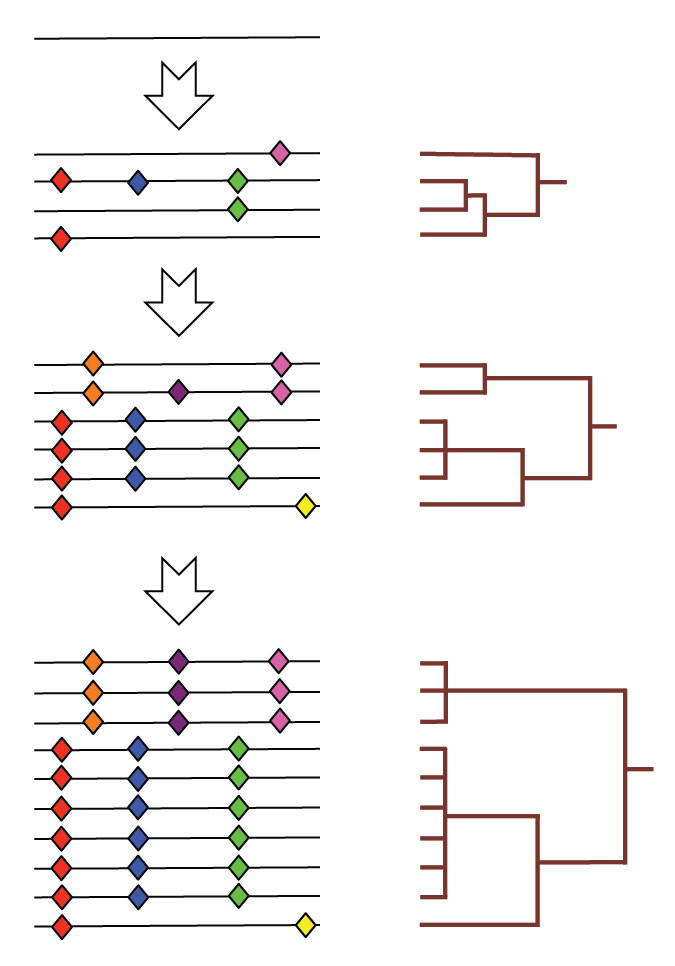
\includegraphics[height=3in]{figures/ClonalEvolutionTrees.png}
    \caption{Left}
    \end{subfigure}
    ~
    \begin{subfigure}{0.5\linewidth}
    \centering
    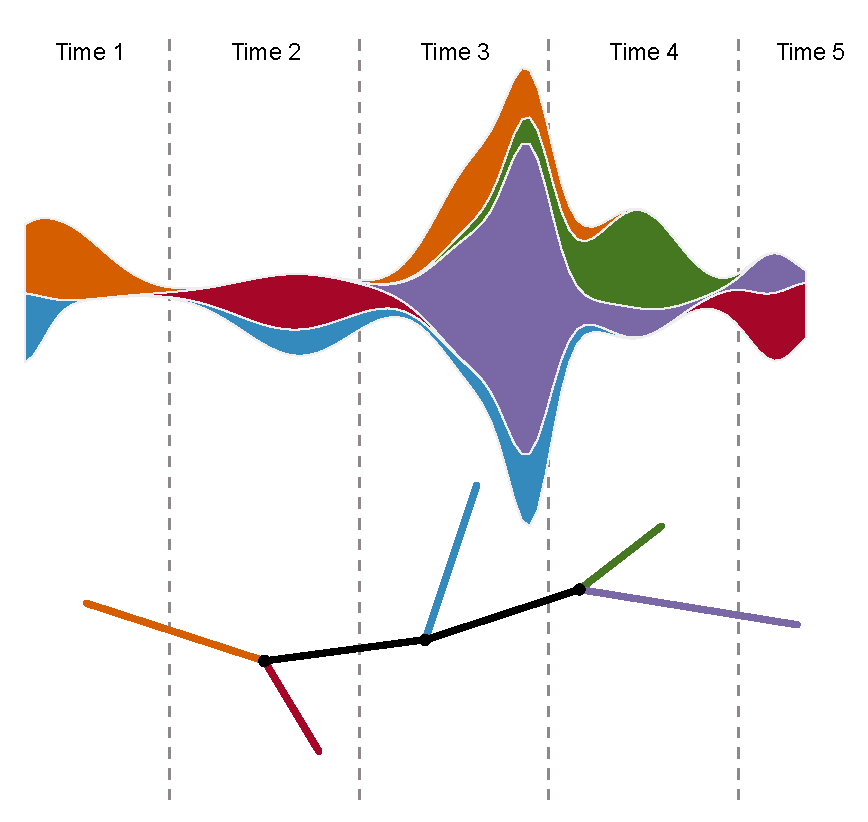
\includegraphics[height=3in]{figures/cartoon_1.pdf}
    \caption{Right}
    \end{subfigure}
    \caption{Clonal evolution of an asexually reproducing organism. (a) Through acquiring mutations and differentiation, the primordial clonal gives rise to a large heterogeneous population, whose evolution can be described with tree-like structures. (b) Longitudinal sampling of a clonal population permits the construction of phylogenetic trees that describe its evolutionary history. Here, sub-populations are represented by different colors; sub-sampling of a particular sub-population is illustrated by the color of the branch in the tree, one of the many trees that can be reconstructed from this population. }
     \label{fig:cartoon_1}
\end{figure}


\begin{figure}
    \centering
    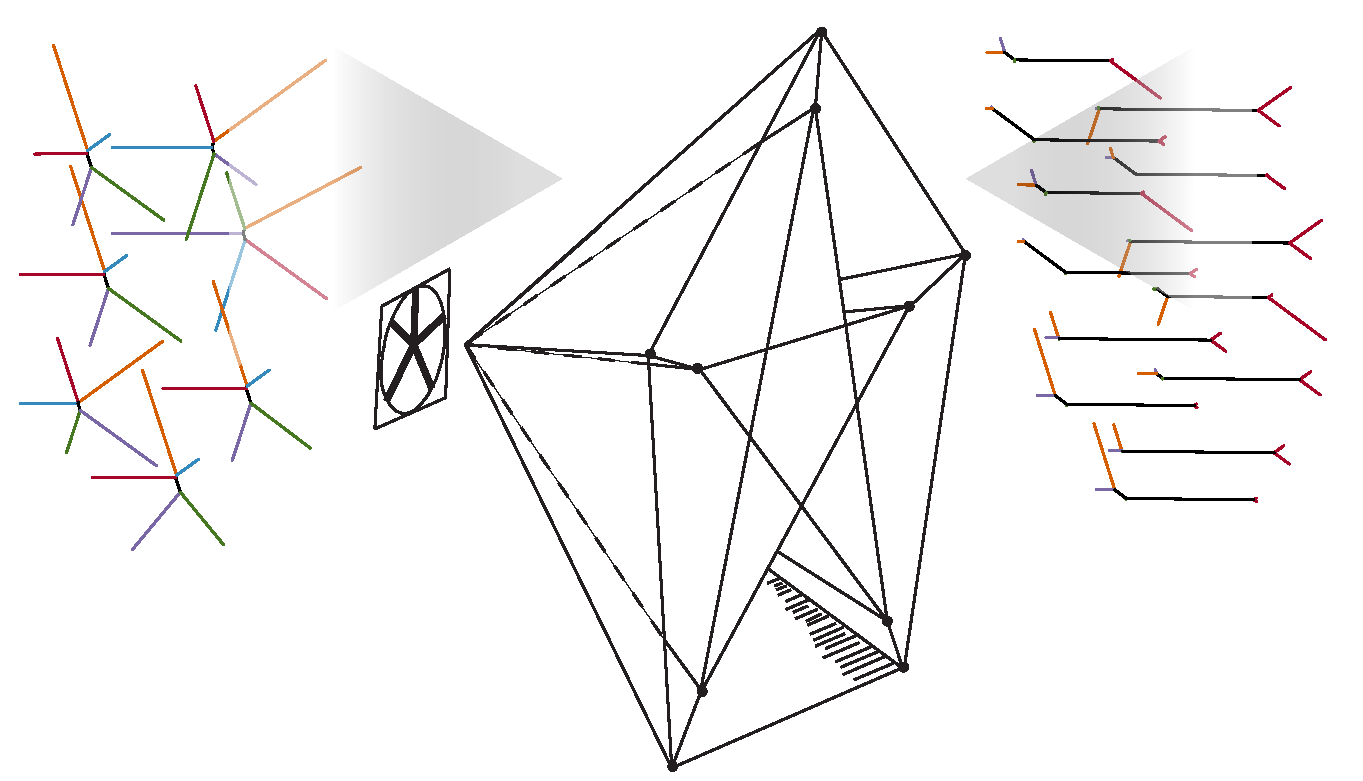
\includegraphics[height=3in]{figures/cartoon_2.pdf}
    \caption{Comparing the evolution of clonal populations by mapping their phylogenetic tree onto the evolutionary moduli space.}
    \label{fig:cartoon_2}
\end{figure}

These and many other questions associated with clonal processes can be expressed in terms of comparing  evolutionary histories.
For instance, stratifying patients according to their evolutionary history requires a way of comparing trees and associating statistics to their ``distances.''
In a recent paper~\cite{zairis2014moduli}, we suggested a simple strategy to construct and study the properties of the space of all potential evolutionary histories, where each history/patient is represented by a point  [REF] \ref{fig:cartoon_2}. We referred to these spaces as  ``evolutionary moduli spaces'' in which classifying histories translates into finding patterns within a point cloud.

In this manuscript,  we present a set of techniques that allow machine learning, tree dimensionality reduction, and statistical inference in ``evolutionary moduli  spaces.''
In Section~\ref{sec:phylospace}, we rapidly review some of the fundamental notions regarding the geometry of evolutionary moduli spaces, following Billera-Holmes-Vogtman \cite{billera2001geometry}, Sturm \cite{sturm2003probability}, and our prior work \cite{zairis2014moduli}. 
Motivated by several biological applications, we will introduce a projective version of these spaces and study some of their geometric properties.
In Section~\ref{sec:ML}, we give an overview of the application of standard machine learning and statistical inference techniques in these spaces. 
In Section~\ref{sec:treedimred}, we will also introduce the concept of ``tree dimensionality reduction'' as a means to visualize and study densely populated trees. 
In Section~\ref{sec:simulated}, we evaluate our methodology using synthetic data, and In the last two chapters, we will discuss two sets of biologically relevant examples.
In Section~\ref{sec:cancer}, we report the predictive power of evolutionary moduli spaces using cancer genomic data, and in Section~\ref{sec:flu}, we study complex trees whose lower dimensional projections readily represent and capture interesting biological phenomena such as clonal replacement events.
%%In our first example, we study how therapy disrupts the linear evolutionary process of chronic lymphocytic leukemias.
%%The second examples shows how patients whose gliomas evolve in a similar fashion present similar grade in later phases of the disease.
%The first example deals the evolution of the hemagglutinin gene of influenza A in humans.
%In our second example we study data from single cell genomics in cancer.

%%%%%%%%%%%%%%%%%%%%%%%%%%%%%%%%%%%%%%%%%%%%%%%%%%%%%%%%%%%%%%%%%%%%%%%%%%%%%%%%%%%%%%%%%%%%%%%%%%%%
%%%%%%%%%%%%%%%%%%%%%%%%%%%%%%%%%%%%%%%%%%%%%%%%%%%%%%%%%%%%%%%%%%%%%%%%%%%%%%%%%%%%%%%%%%%%%%%%%%%%

\section{Spaces of phylogenetic trees}\label{sec:phylospace}

The foundation of our framework for analysis is the {\em metric geometry} of the space of phylogenetic trees.
The purpose of this section is to describe in detail the spaces of phylogenetic trees and their geometric structure.
We begin with a rapid review of the geometry of metric spaces.
We then review the definition and properties of the Billera-Holmes-Vogtmann metric space of phylogenetic trees and its metric geometry.
Finally, we describe the structure of the projective tree space that is our main focus.
In particular, we explain how to compute the induced metric.

\subsection{A rapid review of metric geometry}

A metric space $(X,d)$ is a set $X$ equipped with a distance function $d \colon X \times X \to \mathbb{R}^{\geq 0}$ satisfying the properties that $d(x,y) = d(y,x)$, $d(x,y) = 0$ if and only if $x = y$, and $d(x,z) \leq d(x,y) + d(y,z)$ for all $x,y,z \in X$.
Although metric spaces often arise in contexts in which there is not an evident notion of geometry, it turns out that under very mild hypotheses a metric space $(X,d)$ can be endowed with structures analogous to those arising on Riemannian manifolds.
A metric space $(X,d)$ is a geodesic metric space if any two points $x$ and $y$ can be joined by a path with length precisely $d(x,y)$.
A key insight of Alexandrov observed that is that a good notion of {\em curvature} makes sense in any geodesic metric space~\cite{alexandrov1957uber}.

The idea is that the curvature of a space can be detected by considering the behavior of the area of triangles, and triangles can be defined in any geodesic metric spaces.
Specifically, given points $p, q, r$, we have the triangle $T = [p,q,r]$ with edges the paths that realize the distances $d(p,q)$, $d(p,r)$, and $d(q,r)$.
The connection between curvature and area of triangles comes from the observation that given side lengths $(\ell_1, \ell_2, \ell_3) \subset \mathbb{R}^3$, a triangle with these side lengths on the surface of the Earth is ``fatter'' than the corresponding triangle on a Euclidean plane.
To be precise, we consider the distance from a vertex of the triangle to a point $p$ on the opposite side --- in a fat triangle, this distance will be larger than in the the corresponding Euclidean triangle. (Thin triangles are defined analogously.)

Given a triangle $T=[p,q,r]$ in $(X,d)$, we can find a corresponding triangle $\tilde{T}$ in Euclidean space with the same edge lengths.
Given a point $z$ on the edge $[p,q]$, a comparison point in $\tilde{T}$ is a point $\tilde{z}$ on the corresponding edge $[\tilde{p}, \tilde{q}]$ such that $d(\tilde{z}, \tilde{p}) = d(p,z)$.
We say that a triangle $T$ in $M$ satisfies the $\CAT(0)$ inequality if for every pair of points $x$ and $y$ in $T$ and comparison points $\tilde{x}$ and $\tilde{y}$ on $\tilde{T}$, we have $d(x,y) \leq d(\tilde{x}, \tilde{y})$.
If every triangle in $M$ satisfies the $\CAT(0)$ inequality then we say that $M$ is a $\CAT(0)$ space.

More generally, let $M_{\kappa}$ denote the unique two-dimensional Riemannian manifold with curvature $\kappa$.
The diameter of $M_{\kappa}$ will be denoted $D_{\kappa}$.
Then we say that a $D_{\kappa}$-geodesic metric space $M$ is $\CAT(\kappa)$ if every triangle in $M$ with perimeter $\leq 2D_{\kappa}$ satisfies the inequality above for the corresponding comparison triangle in $M_{\kappa}$.
If $\kappa' \leq \kappa$, any $CAT(\kappa')$ space is also $\CAT(\kappa)$.
A $n$-dimensional Riemannian manifold $M$ that is sufficiently smooth has sectional curvature $\leq \kappa$ if and only if $M$ is $\CAT(\kappa)$.
For example, Euclidean spaces are $\CAT(0)$, spheres are $\CAT(1)$, and hyperbolic spaces are $\CAT(-1)$.

As described, $\CAT(\kappa)$ is a global condition; we will say that a metric space $(X,d)$ is locally $\CAT(\kappa)$ if for every $x$ there exists a radius $r_x$ such that $B_{r_x}(x) \subseteq X$ is $\CAT(\kappa)$.
For example, the flat torus is locally $\CAT(0)$ but not globally $\CAT(0)$.
The Cartan-Hadamard theorem implies that a simply-connected metric space that is locally $\CAT(0)$ is also globally $\CAT(0)$.

A remarkably productive observation of Gromov is that many geometric properties of Riemannian manifolds are shared by $CAT(\kappa)$ spaces.
In particular, $\CAT(\kappa)$ spaces with $\kappa \leq 0$ (referred to as {\em non-positively curved metric spaces}) admit unique geodesics joining each pair of points $x$ and $y$, balls $B_{\epsilon}(x)$ are convex and contractible for all $x$ and $\epsilon \geq 0$, and midpoints of geodesics are well-behaved.
As a consequence, there exist well-defined notions of mean and variance of a set of points, and more generally one can attempt to perform statistical inference, as we explain below.

\subsection{Cubical complexes and their links}

In this section, we review the theory of cubical complexes, which provide a rich source of examples of $\CAT(0)$ metric spaces.
It is in general very difficult to determine for an arbitrary metric space whether it is $\CAT(\kappa)$ for any given $\kappa$.
Even for finite simplicial complexes, this problem does not have a general solution.
The important of cubical complexes comes from an effective criterion for determining if they are non-positively curved.

Let $I^n$ denote the $n$-dimensional unit cube $[0,1] \times \ldots \times [0,1]$, regarded as inheriting a metric structure from the standard metric on $\mathbb{R}^n$.
A codimension $k$ face of the cube $I^n$ is determined by fixing $k$ coordinates to be in the set $\{0,1\}$.
A cubical complex is a metric space obtained by glueing together cubes via the data of isometries of faces, subject to the condition that two cubes are connected by at most a single face identification and no cube is glued to itself.
The metric structure is the length metric induced from the Euclidean metric on the cubes, i.e., the distance between $x$ and $y$ is the infimum of the lengths over all paths from $x$ to $y$ that can be expressed as the union of finitely many segments each contained within a cube.
When the cubical complex $C$ is finite or locally finite, results of Bridson and Moussong imply that $C$ is a complete geodesic metric space.

Gromov gave a criterion for a cubical complex to be $\CAT(0)$ that is often possible to check in practice.
In order to explain this criterion, we need to review the notion of the link of a vertex in a cubical complex.

Fix a vertex $v$ in a cubical complex $C$ and a cube $C_i \cong I^m \subseteq C$ such that $v$ is a vertex of $C_i$.
For fixed $\epsilon > 0$, the all-right spherical simplex associated to $(C_i,v)$ is the subset $S(C_i,v) = \{z \in C_i \, | \, d(z,v) = \epsilon\}$.
The set $S(C_i,v)$ has a metric induced by the Euclidean angle metric.
The faces of $S(C_i,v)$ are defined as the intersections of $S(C_i,v)$ with faces of $C_i$; equivalently, these are the all-right spherical simplexes associated to faces of $C_i$.
The collection of all-right spherical simplices for all pairs $(C_i, v)$ forms a polyhedral complex with metric given by the length metric induced from the angle metrics; this is referred to as a spherical complex.
Forgetting the metric structure, the all-right spherical simplices also form an abstract simplicial complex. (Recall that an abstract simplicial complex is simply a set of subsets of a set $V$ that is closed under passage to subsets.)

The link of a vertex $v$ in a cubical complex $C$ is the spherical complex obtained as the subset $L(v) = \{z \in C \, | \, d(z,v) = \epsilon\}$, for fixed $0 < \epsilon < 1$.
Gromov's criterion now states that the cubical complex $C$ is locally $\CAT(0)$ if and only if the link is $\CAT(1)$ or the abstract simplicial complex underlying the link is flag.
(Recall that a flag complex is a simplicial complex in which a $k$-simplex is in the complex if and only its $1$-dimensional faces are in the complex.)

As an easy application of Gromov's criterion, we conclude the section by showing that the cartesian product of locally $\CAT(0)$ cubical complexes is itself a locally $\CAT(0)$ cubical complex.
Let $X$ and $Y$ be cubical complexes that are $\CAT(0)$.
Since $I^n \times I^m \cong I^{n+m}$, it is clear that $X \times Y$ has the structure of a cubical complex.
The set of vertices of $X \times Y$ is given by the product of the sets of vertices of $X$ and $Y$ respectively.
The link of a vertex $(v,v')$ in $X \times Y$, regarded as an abstract simplicial complex, is the join of $L(v)$ and $L(v')$, which we denote $L(v) \ast L(v')$.
(The join of complexes $S_1$ and $S_2$ is obtained by considering all pairwise unions of elements of $S_1$ and $S_2$.)
Finally, since the join of flag complexes is easily seen to be a flag complex, Gromov's criterion now implies that $X \times Y$ is locally $\CAT(0)$.

\subsection{The Billera-Holmes-Vogtmann spaces of phylogenetic trees}

A phylogenetic tree with $m$ leaves is a weighted, connected graph with no circuits, having $m$ distinguished vertices of degree $1$ labeled $\{1, \ldots, m\}$ (referred to as {\em leaves}), and all other vertices of degree $\geq 3$.
We refer to edges that terminate in leaves as {\em external} edges and the remaining edges are {\em internal}.

The space $\BHV_m$ of isometry classes of rooted phylogenetic trees with $m$-labelled leaves where the nonzero weights are on the internal branches was introduced and studied by Billera, Holmes, and Vogtmann.
The space $\BHV_n$ is constructed by gluing together $(2n-3)!!$ positive orthants $\mathbb{R}^n_{\geq 0}$; each orthant corresponds to a particular tree topology, with the coordinates specifying the lengths of the edges.
Allowing potentially nonzero weights for the $m$ external leaves corresponds to taking the cartesian product with an $m$-dimensional orthant.
We will focus on the space 
\[\Sigma_m = \BHV_{m-1} \times (\mathbb{R}^{\geq 0})^{m},\]
which we refer as the evolutionary moduli space.
(The $m-1$ index arises from the fact that we consider unrooted trees.)

The main result of Billera, Holmes, and Vogtmann is that the length metric on $\BHV_n$ endows this space with a (global) $\CAT(0)$ structure.
The metric on $\BHV_{m-1}$ is induced from the standard Euclidean distance on each of the orthants, as follows.
For two trees $t_1$ and $t_2$ which are both in a given orthant, the distance $d_{\BHV_{m-1}}(t_1,t_2)$ is defined to be the Euclidean distance between the points specified by the weights.
For two trees which are in different quadrants, there exist (many) paths connecting them which consist of a finite number of straight lines in each quadrant.
The length of such a path is the sum of the lengths of these lines, and the distance $d_{\BHV_{m-1}}(t_1,t_2)$ is then the minimum length over all such paths.
There is an analogous metric on $\Sigma_m$, which can be regarded as induced from the metric on $\BHV_{m-1}$.
Specifically, for a tree $t$, let $t(i)$ denote the length of the external edge associated to the vertex $i$.
Then \[d_{\Sigma_m}(t_1,t_2) = \sqrt{d_{\BHV_{m-1}}(\bar{t}_1,\bar{t}_2) + \sum_{i=1}^m (t_1(i) - t_2(i))^2},\] where $\bar{t}_i$ denotes the tree in $\BHV_{m-1}$ obtained by forgetting the lengths of the external edges (e.g., see~\cite{owen2011fast}).

By subdividing each orthant into cubes in the evident fashion, $\Sigma_m$ is naturally a cubical complex where the metric we have described is the one induced from the Euclidean metric on the cubes.
Now a straightforward combinatorial analysis of the link of $\Sigma_m$ implies the following theorem via Gromov's criterion.

\begin{theorem}[{\cite[4.1]{billera2001geometry}}]
The space $\Sigma_m$ is a $\CAT(0)$ space.
\end{theorem}

In addition, $\Sigma_m$ is clearly a complete metric space.
Furthermore, it is separable, which means that it contains a countable dense subset; any tree can be approximated by a sequence of trees in the same orthant that have rational edge lengths.
A complete and separable metric space is called a Polish space; on such metric spaces, the usual probabilistic machinery behaves as expected.

\begin{theorem}
The space $\Sigma_m$ is a Polish space.
\end{theorem}

As explained in ~\cite[\S4.2]{billera2001geometry}, efficiently computing the metric on $\Sigma_m$ is a nontrivial problem.
We will rely on the fact that there exists a polynomial-time algorithm based on successive approximation of geodesic paths~\cite{owen2011fast}.

\subsection{The projective evolutionary moduli space}

We are primarily interested in classifying and comparing distinct evolutionary behaviors by understanding the relative lengths of edges: rescaling edge lengths should not change the relationship between the branches.
This leads us to consider the quotient space of $\Sigma_m$ by the equivalence relation that for each orthant, the tree $\{t_i\}$ is equivalent to the rescaled tree $\{\lambda t_i\}$.
That is, we define $\mathbb{P} \Sigma_m$ to be the subspace of $\Sigma_m$ consisting of the points $\{t_i\}$ in each orthant for which the constraint $\sum_{i} t_i = 1$ holds.

The space of trees with internal edges of fixed length was studied by Boardman and is denoted by $\tau_{m-1}$.
The space of $m$ external branches whose lengths sum to $1$ is the standard $m-1$ dimensional simplex $\Delta_{m-1}$ in $\mathbb{R}^m$.
In terms of these spaces, the requirement that the length of internal branches plus the external branches sum to $1$ implies that
\[\mathbb{P}\Sigma_m = \tau_{m-1} \star \Delta_{m-1}.\] 
Alternatively, we can describe $\mathbb{P}\Sigma_m$ as the link on the origin in $\Sigma_m$.

There are various possible natural metrics to consider on $\mathbb{P} \Sigma_m$.
The simplest way to endow $\mathbb{P} \Sigma_m$ with a metric is to use the subspace metric.
The subspace metric is also very natural from the perspective of our applications.
However, from the perspective of metric geometry, the characterization of $\mathbb{P} \Sigma_m$ as the link of the origin endows it with the structure of an all-right spherical complex.
Gromov's theorem then implies that with this metric, $\mathbb{P} \Sigma_m$ is a $\CAT(1)$ space.
Furthermore, it is clear that with either of these metrics, $\mathbb{P} \Sigma_m$ is a Polish space.

Since neither metric on $\mathbb{P} \Sigma_m$ makes it into a $\CAT(0)$ space, the problem of efficiently computing the metric becomes more acute.
We approach this problem by using $\epsilon$-nets and a local-to-global construction.
Recall that a set of points $S$ in a metric space $(X,\partial)$ is an $\epsilon$-net if for every $z \in X$, there exists $q \in S$ such that $\partial(z,x) < \epsilon$.
For a compact metric space equipped with a probability measure such that all non-empty balls in the metric space have nonzero measure, we can produce an $\epsilon$-net by sampling.
More precisely, it is straightforward to show that given a finite collection of measurable sets $\{A_1, A_2, \ldots, A_k\}$ and a probability measure $\mu$ on $\cup_i A_i$ such that $\mu(A_i) \geq \alpha > 0$, then given at least 
\[
\frac{1}{\alpha}\left(\log k + \log(\frac{1}{\delta})\right)
\]
samples, with probability $1-\delta$ there is at least one sample in every $A_i$~\cite[5.1]{niyogi2008finding}.

Next, suppose that we have a metric space $(X,\partial)$ where there exists a constant $\kappa$ such that if $\partial(x,y) < \kappa$, it is easy to compute $\partial(x,y)$.
An algorithm for approximating $\partial$ on all of $X$ is then to take a dense sample $S \subset X$, form the graph $G$ with vertices the points of $S$ and edges between $x$ and $y$ when $\partial(x,y) < \kappa$, and define the distance between $x$ and $y$ in $X$ to be the graph metric on $G$ between the nearest points to $x$ and $y$ in $S$.
This distance can be efficiently computed using Djikstra's algorithm.

When $S$ is an $\epsilon$-net for sufficiently small $\epsilon$ relative to $\kappa$, we can describe the quality of the resulting approximation to $\partial$~\cite[Thm. 2]{bernstein2000graph}.
In particular, if $\epsilon < \frac{\kappa}{4}$, then 
\[
\partial(x,y) \leq \partial_G(x,y) \leq (1 + 4\frac{\delta}{\epsilon}) \partial(x,y).
\]

Putting this all together, to approximate the metric on $\mathbb{P}\Sigma_m$ we take the union of $\epsilon$-nets on all of the simplices (including the faces) and form a $\kappa$-approximation $\partial_G$ as above.
In practice, the required density of samples is determined by looking at when the approximation converges (i.e., when the change in distances drops below a specified precision bound).

\subsection{The injectivity radius in $\mathbb{P}\Sigma_m$}

Since $\Sigma_m$ is a $\CAT(0)$ space, any two points are connected by a unique geodesic.
In contrast, $\mathbb{P}\Sigma_m$ does not have this property in either of the metrics discussed above.
In the spherical metric, $\mathbb{P}\Sigma_m$ is a $\CAT(1)$ space; as a consequence, there is a finite injectivity radius, which is the maximum distance between points $p,q \in \aP_n$ such that the distance between $p$ and $q$ is realized by a unique geodesic.
The subspace metric (which is a ``flattening'' of the spherical metric) also fails to have unique realizations for the distances between all points.

We now explain where the non-unique geodesics in $\mathbb{P}\Sigma_m$ come from.
For simplicity, we will focus on the link in $\BHV_m$, which we will denote by $\aP_m$, and temporarily ignore the join with the simplex coming from the external edge lengths.
Observe that adjacent top-dimensional simplices in $\aP_m$ differ by a {\em rotation} of tree topologies, where a rotation collapses an internal edge and then expands out from the resulting node.
Next, recall that the homotopy type of $\aP_n$ is a wedge of $(n-1)!$ spheres of dimension $(n-3)$~\cite{robinson1996tree} (and see also~\cite[Thm. 6]{devadoss2014polyhedral}).
Moreover, we can explicitly describe these spheres, as follows.

As discussed in~\cite[Prop. 1]{devadoss2014polyhedral} and~\cite[\S 3.1]{billera2001geometry}, the boundary of the dual polytope to standard associahedron on $n$ letters (parametrizing parenthesizations of $n$ terms) embeds in many different ways into $\aP_n$.
Following~\cite{devadoss2014polyhedral}, let us denote this boundary by $\aK_n$.
Explicitly $\aK_n$ is a simplicial sphere of dimension $(n-3)$ where a $k$-simplex corresponds to a planar rooted tree with $n$ leaves and $k+1$ internal edges.
Then the homotopy type of $\aP_n$ can be described in terms of various embedded copies of $\aK_n$.
As a consequence, to understand the injectivity radius of $\aP_n$, we need to compute the diameter of $\aK_n$.

For convenience, we describe this diameter in terms of counts of simplices; the actual value can then be obtained by multiplying by the diameter of a simplex.
In this guise, the problem is an old one which can be described in many different forms, perhaps most relevantly as the computation of maximal rotation distances between binary trees.

The main result here is that the diameter of $\aK_n$ is $2n - 8$ for $n > 11$~\cite{pournin2014diameter}; this bound was established asymptotically (for sufficiently large but indeterminate $n$) in~\cite{sleator1988rotation}.
For smaller values, we have the following table (taken from~\cite[\S2.3]{sleator1988rotation}) of explicit values:

\begin{table}[ht]
    \caption{Diameters for $\aK_n$ for small values of $n$}
    \centering
    \begin{tabular}{c c c c c c c c}
    \hline\hline
    4 & 5 & 6 & 7 & 8 & 9 & 10 & 11 \\
    \hline
    2 & 4 & 5 & 7 & 9 & 11 & 12 & 15 \\
    \hline
    \end{tabular}
\end{table}

\begin{warning}
The results given in~\cite{pournin2014diameter} and~\cite{sleator1988rotation} differ slightly from the formula above and from each other due to divergent choices of indexing convention about precisely what $n$ means.
\end{warning}

Unfortunately, computing the rotation distance is not known to have a polynomial-time solution, but there are efficient approximation algorithms (all of which have an error bound around $2$) that operate in linear time~\cite{cleary2010linear}.

Returning to the case of $\mathbb{P}\Sigma_m$, the join with the standard simplex adds further complication; paths that realize the distance may involve motion in the cone coordinate as well as in the ``rotation'' direction.
In practice, we can determine if two points are connected by a unique geodesic by repeated use of Djikstra's algorithm in $G$; after finding the shortest path, we can successively form graphs $G'$ by removing edges and then using Djikstra's algorithm on $G'$.

\subsection{Binary trees and triangulations of convex polygons}

Two trees $T_1$ and $T_2$ are in adjacent orthants of $\Sigma_m$ when they are related by a rotation, which we described above as the transformation on a tree performed by collapsing a specified edge to one of its incident vertices and then expanding out an edge from that vertex.
In order to study the geometry of tree space, it is often useful to have an alternate description of the rotation operation.
We now explain the connection between binary trees and triangulations of convex polygons; in the setting of polygons, the rotation operation has a simple geometric description.
This model was used in the computation of the diameter in rotation distance of tree space described above, and will be applied below when we study tree dimensionality reduction~\ref{sec:treedimred}.

Given a triangulation of a convex polygon with $n$ vertices, the dual graph is formed by taking a vertex for each triangle and an edge connecting vertices in adjacent triangles.
It is clear that the dual graph forms a binary tree.
On the other hand, given a rooted binary tree with $n$ leaves, we can recursively produce a triangulation of the regular $n+1$-gon as follows.
We label the edges of the polygon by the leaves in counterclockwise order.  
We then add the triangle formed by the edge corresponding to the root of the tree and the vertex $k+3$, where $k$ denotes the number of leaves on the left side of the root.
The process is then recursively carried out on the two polygons formed by this triangle.

A rotation of a tree in this context is now specified by choosing a quadrilateral formed by two adjacent triangles and ``flipping the diagonal''; i.e., deleting the diagonal chord and replacing it with the diagonal through the two vertices the original diagonal did not use.
(It is straightforward to check that this corresponds to the rotation operation on binary trees.)

%%%%%%%%%%%%%%%%%%%%%%%%%%%%%%%%%%%%%%%%%%%%%%%%%%%%%%%%%%%%%%%%%%%%%%%%%%%%%%%%%%%%%%%%%%%%%%%%%%%%
%%%%%%%%%%%%%%%%%%%%%%%%%%%%%%%%%%%%%%%%%%%%%%%%%%%%%%%%%%%%%%%%%%%%%%%%%%%%%%%%%%%%%%%%%%%%%%%%%%%%

\section{Machine learning and statistical inference in $\Sigma_m$ and $\mathbb{P}\Sigma_m$}\label{sec:ML}

The motivation for characterizing the metric geometry of $\Sigma_m$ and $\mathbb{P}\Sigma_m$ comes from the problems of describing and comparing collections of trees generated from experimental data.
Regarding such collections as samples from distributions on the evolutionary moduli spaces, we are interested in basic statistical inference --- estimating parameters describing these distributions and determining if two samples came from the same or different distributions.
More generally, we would like to understand the kinds of distributions that can arise in evolutionary moduli spaces.
We are also interested in clustering and classification (i.e., unsupervised and supervised learning) problems in this context.
Given a set of unlabeled samples, we want to infer clusters of points that have similar clinical outcomes.
Given a set of labeled samples, we want to produce classifiers that can assign labels to new points in order to predict clinical outcomes.

\subsection{Statistics for distributions in $\Sigma_m$ and $\mathbb{P}\Sigma_m$}

In contrast to classical statistics on $\mathbb{R}^n$, we do not know many sensible analytically-defined distributions on the evolutionary moduli spaces.
Billera-Vogtmann-Holmes briefly introduce a family of Mallows distribution on $\Sigma_m$ with density function
\[
x(t) = \kappa e^{\alpha d_{\Sigma_m}(t_1, t)}
\] 
for fixed $t_1 \in \Sigma_m$, and an analogous family can be defined on $\mathbb{P}\Sigma_m$.
Sampling from these distributions is somewhat subtle; the natural approach is to use a Markov chain Monte Carlo (MCMC) algorithm, but convergence for such chains is not well-understood and can have pathological behavior near the origin (due to the explosion in the number of trees within an $\epsilon$ ball).
{\bf Say something here about rotation walk.}

A much more tractable source of distributions on $\Sigma_m$ and $\mathbb{P}\Sigma_m$ arise from resampling from a given set of empirical data points.
However, as we discuss below, since the central limit theorem in nonpositively curved metric spaces can be quite complicated, once again our understanding of the behavior of resampling estimators is incomplete.

In order to study probability distributions in evolutionary moduli spaces, it is necessary to have reasonable notions of moments of the distribution, expectation of random variables, and analogues of the law of large numbers.
Since $\Sigma_m$ is a $\CAT(0)$ space, points are connected by unique geodesics and there is a sensible notion of a centroid of a collection of points.
Indications of the use of these properties for statistical inference in $\Sigma_m$ were given in~\cite{billera2001geometry}, and subsequently Holmes has written extensively on this topic~\cite{holmes2003bootstrapping, holmes2003bootstrapping, holmes2005statistical} (and see also~\cite{feragen2013tree}).
More generally, an account of probability measures on general $\CAT(0)$ spaces has been given by Sturm~\cite{sturm2003probability}.
The approach taken there specifies the sample mean and variance of a set of points in $\Sigma_m$ in terms of a generalization of a centroid: we define the Fr\'echet mean and variance in $\Sigma_m$.

\begin{definition}
Given a fixed set of $n$ trees $\{T_0, \ldots T_{n-1}\} \subseteq \Sigma_m$, the Fr\'echet mean $T$ is the unique tree that minimizes the quantity \[E = \sum_{i = 0}^{n-1} d_{\Sigma_m}(T_i, T)^2.\] 
The variance of $T$ is the ratio $\frac{E}{n}$.
\end{definition}

Sturm's work provides an iterative procedure for computing the mean and variance of a set of points in $\Sigma_m$, and by exploiting the local geometric structure of $\Sigma_m$, Miller, Owen, and Provan produce somewhat more efficient algorithms for computing the mean~\cite{miller2012polyhedral}.
Furthermore, Sturm proves versions of Jensen's inequality and the law of large numbers in this context.
Barden, Le, and Owen study central limit theorems for Fr\'echet means in $\Sigma_m$~\cite{barden2013mean}; as they explain, the situation exhibits non-classical behavior and the limiting distributions depend on the codimension of the simplex in which the mean lies.
Finally, there has been some work on principal components analysis (PCA) in $\Sigma_m$; the resulting algorithms are computationally involved and fail to capture much of the variance~\cite{Nye2011PCA}.

The situation for $\mathbb{P}\Sigma_m$ is substantially more complicated.
The failure of the existence of unique geodesics between points means that the Fr'echet mean is not unique and so the associated variance can be discontinuous in small perturbations of the points.
Only when the diameter of the set of sample points is smaller than the injectivity radius do we expect consistent behavior from these moments.
When working in $\mathbb{P}\Sigma_m$, we have found it useful to consider the alternate summary tree produced by hierarchical clustering; while in no sense an ``average tree'', the resulting tree does capture information about the metric structure of a finite set of points.

\subsection{Distributions in $\Sigma_m$ and $\mathbb{P}\Sigma_m$ via distributions in $\mathbb{R}^n$}

One way to grapple with the difficulties in dealing with distributions on $\Sigma_m$ and $\mathbb{P}\Sigma_m$ is to instead study associated projections into distributions on Euclidean space.
The advantage of this approach is evident; we are now in a setting where the theory of moments, the central limit theorem, and asymptotic consistency for resampling procedures are all very familiar.
Of course, it is important to keep in mind that the moments derived in this setting will reflect the geometry of the evolutionary moduli space is complicated ways, and inverses to the projections will not usually exist.
Nonetheless, for purposes of many kinds of statistical tests (e.g., hypothesis testing about distributions generating observed samples), this approach can be very effective.
There are a number of natural ways to map metric measure spaces into Euclidean space; in this section, we discuss several strategies derived from the use of the metric.

An intrinsic map comes from looking at the distance distribution on $\mathbb{R}$ induced by $\partial_M$.
Specifically, given a Borel distribution $\Psi$ on $(M, \partial_M)$, the product distribution $\Psi \otimes \Psi$ on $M \times M$ induces a distibution on $\mathbb{R}$ via $\partial_M$.
Applying this construction to the empirical measure on a finite sample yields the empirical distance distribution.
More generally, for any fixed $n$, we can consider the distribution on $\mathbb{R}^{n^2}$ induced by taking the product distribution $\Psi^{\otimes n}$ on $M^{\times n}$ and applying $\partial_M$ to produce the $n \times n$ matrix of distances.
Gromov's ``mm-reconstruction theorem'' showed that in the limit as $n \to \infty$, the distance matrix distributions completely characterize the distribution $\Psi$ on $(M, \partial_M)$~\cite{gromov1981}.
Once again, given a sufficiently large finite sample, we can construct the empirical distance matrix distributions for any fixed $n$.

Another approach involves choosing a fixed set of $n$ landmarks and considering the vector of distances from a fixed point to the landmarks.
Given a set $L = \{t_1, t_2, \ldots, t_n\} \subset $, there is a continuous map
\[
d_L \colon M \to \mathbb{R}^n
\]
specified by
\[
x \mapsto (\partial_M(x,t_1), \partial_M(x,t_2), \ldots, \partial_M(x,t_n)).
\]
Pushforward along $d_L$ again induces a distribution on $\mathbb{R}^n$ from one on $M$.
One expects that as $k$ increases (provided the landmarks are ``generic''), the induced distributions in $\mathbb{R}^n$ will characterize the distribution on $M$.

In both cases, choice of the parameter $k$ depends on some sense of the intrinsic dimension of the support of the distribution as well as the number of points available (in the case of finite samples).
Unfortunately, the required $k$ may well be quite large.
{\bf Explain example of wedge of circles.}
In our work, we use cross-validation techniques to determine suitable $k$, as discussed below.

Finally, there is a substantial body of work on low-distortion embeddings of finite metric spaces into $\ell^p$ spaces, in particular Euclidean spaces.
Recall that the distortion of a non-contractive (distance expanding) embedding of metric spaces $f \colon (X, \partial_X) \to (Y, \partial_Y)$ is given by $\sup_{x_1 \neq x_2} \frac{\partial_Y (f(x_1), f(x_2))}{\partial_X (x_1, x_2)}$. 
Notably, Abraham, Bartal, and Neiman show that one can construct a probabilistic embedding of an $n$-point finite metric space into an $O(\log n)$ dimensional space with distortion $O(\log n)$.
Pushing forward distributions on $\Sigma_m$ and $\mathbb{P}\Sigma_m$ provide another way of reducing statistical questions to Euclidean space.

\subsection{Distinguishing samples from different underlying distributions}

Given a set of samples $X \subset \Sigma_m$ and a partition $X = \aC_1 \cup \aC_2 \ldots \cup \aC_n$ (where $\aC_i \cap \aC_j = \emptyset$), it is often useful to be able to determine whether or not the different $\aC_i$ were generated from the same or different underlying distributions.
For instance, $\aC_1$ might represents samples from patients who received treatment and $\aC_2$ is untreated patients, or the different groups $\aC_i$ represent different observed genetic markers.
Based on the discussion of the previous two subsections, we can study this problem directly in $\Sigma_m$ or in via projections to $\mathbb{R}^n$.

When working in $\Sigma_m$, the Fr\'echet mean and variance provides a summary of each collection of samples $\aC_i$.
A standard comparison between groups is then given by the distance 
\[
\theta_{ij} = d_{\Sigma_m}(T(\aC_i), T(\aC_j))
\]
between the means.
In order to understand the variability due to sampling, we can use bootstrap resampling (or more general $k$ out of $n$ resampling without replacement) to generate confidence intervals for the value of $\theta_i$.
(Asymptotic consistency for the bootstrap follows from the fact that the VC dimension of the collections of balls in $\Sigma_m$ and $\mathbb{P}\Sigma_m$ is bounded, via the usual criteria~\cite{Gine1984, Gine1986, Gine1990}.) 
Examples of this are presented below.{\bf Forward pointer here.}

In contrast, when working in $\mathbb{P}\Sigma_m$, we have no choice to consider tests induced by the projections into $\mathbb{R}^n$ discussed above.
Here, we can compare collections $\aC_i$ and $\aC_j$ by using any of the many standard non-parametric comparison techniques for real distributions, for example $\chi^2$ tests or two-sample Kolmogorov-Smirnov tests.
Again, we present examples of this below.  {\bf Forward pointer here.}

One pervasive problem in clinical applications is that often the number of samples is quite small, and so we are often far from the asymptotic regime for statistical tests.
Standard small-sample corrections can be applied.
However, for this reason a machine learning approach to analyzing the data is often more useful.

\subsection{Clustering in $\Sigma_m$ and $\mathbb{P}\Sigma_m$}

Given the difficulties with statistical inference in $\Sigma_m$ and $\mathbb{P}\Sigma_m$, it is useful to complement these approaches with techniques from machine learning.
The most basic family of techniques we might consider is clustering, a kind of unsupervised learning.
Here, given a finite set $X$ in $\Sigma_m$ or $\mathbb{P}\Sigma_m$, we search for a partitionings of the points into clusters which optimize some criterion for the ``goodness'' of the clustering.

Regarding $\Sigma_m$ and $\mathbb{P}\Sigma_m$ simply as metric spaces, we can apply standard clustering algorithms that operate on arbitrary metric spaces.  
The simplest of these is the $k$-medoids algorithm.
Like $k$-means, $k$-medoids seeks partitions which are optimal in the sense of minimizing the sum of squared distances; the cost function for a cluster $C = \{x_i, x_j\}$ is given by $\sum_{i < j} \partial(x_i,x_j)^2$.
But instead of using cluster centroids as in $k$-means, cluster assignments are determined by medoids, which are points $z \in C$ that minimize $\sum_i d(z,i)$.
The advantage of $k$-medoids over $k$-means is that the problem of finding a centroid in $\Sigma_m$ or $\mathbb{P}\Sigma_m$ is avoided; of course, in $\Sigma_m$ we can also consider $k$-means.

Another natural family of clustering algorithms comes from spectral clustering techniques.
Recall that spectral clustering can be applied to finite subsets of any metric space; one constructs an embedding into Euclidean space using the graph Laplacian associated to a graph encoding the local metric structure of the set of points and then performs $k$-means clustering.
As such, spectral clustering can be applied both to $\Sigma_m$ and $\mathbb{P}\Sigma_m$.

\subsection{Supervised Learning}

Although clustering algorithms are very useful for exploratory data analysis, for clinical applications we expect that classification problems are more salient.
Specifically, a temporal sequence of tumor samples will be linked with a categorical or numeric label denoting the clinical management of the patient.
We would then like to predict patient outcomes or expect response to treatment using a discriminative supervised learning algorithm operating in $\Sigma_m$ or $\mathbb{P}\Sigma_m$.
Analogous to our use of $k$--medoids clustering for unsupervised grouping, the most basic algorithm for supervised learning is a $k$--nearest neighbor ($k$--NN) predictor.
In this algorithm the predicted label for a given point is generated by taking a majority or weighted vote over the labels of the $k$ nearest trees.
The optimal value of $k$ then specifies an order--$k$ Voronoi tesselation of the space that provides a description of the sizes of the predictive neighborhoods surrounding each element of the data set.

Another possibility is exploit embeddings of the data set into $\mathbb{R}^d$.
There are some subtleties to using such embeddings, however.
Notably, since neither $\Sigma_m$ or $\mathbb{P}\Sigma_m$ are Euclidean spaces (as they are evidently not flat), we do not expect a low-distortion global embedding.
Therefore, we have to use embeddings generated by finite samples.
Specifically, we embed both the labeled training points and the new data into $\mathbb{R}^n$, build classifiers on the training data, and then predict the labels for the new data.
This requires generating a new embedding and re-training for each new input to classify, and it is not clear that this procedure is stable under perturbation of the data.
Furthermore, since it is not possible in general to lift classification boundaries in $\mathbb{R}^d$ back to $\Sigma_m$ or $\mathbb{P}\Sigma_m$, qualitative scientific inference about the learned features is difficult.

Finally, it is possible to embed $\Sigma_m$ and $\mathbb{P}\Sigma_m$ isometrically into certain Banach spaces; in fact, for any metric space, we can consider an embedding into the space of linear functionals specified by the taking each point to the functional $\partial(x,-) - \partial(x_0,-)$, where $x_0$ is an arbitrary point.
Since the Banach space of linear functionals is an $\mathbb{R}$-vector space, one can carry out the support vector classification algorithm directly~\cite{hein2003}.
Once again, it is not straightforward to produce classification boundaries in the original space.


%%%%%%%%%%%%%%%%%%%%%%%%%%%%%%%%%%%%%%%%%%%%%%%%%%%%%%%%%%%%%%%%%%%%%%%%%%%%%%%%%%%%%%%%%%%%%%%%%%%%
%%%%%%%%%%%%%%%%%%%%%%%%%%%%%%%%%%%%%%%%%%%%%%%%%%%%%%%%%%%%%%%%%%%%%%%%%%%%%%%%%%%%%%%%%%%%%%%%%%%%

\section{Tree dimensionality reduction}\label{sec:treedimred}

A difficulty that arises in this framework is the fact that as the number of sequential samples used to generate each tree increases, so does the dimensionality of the evolutionary moduli space.
High-dimensional spaces of trees pose problems both because statistical procedures become more difficult to use and because visualization is impossible.
Thus, we are led to consider strategies for dimensionality reduction.
Previously, we discussed dimensionality reduction techniques that do not preserve the geometric structure of the evolutionary moduli space.

In this section, we describe a technique for dimensionality reduction that projects a single tree in $\Sigma_m$ or $\mathbb{P}\Sigma_m$ onto a set of trees in $\Sigma_{n}$, for $n < m$.
Given a sample in $\Sigma_m$ or $\mathbb{P}\Sigma_m$, applying this projection to each tree yields an expanded sample in $\Sigma_n$.
We believe that the analysis and visualization of the resulting clouds of trees is an effective way to study high-dimensional evolutionary moduli spaces.
To just the use of tree dimensionality reduction, we prove that this procedure is stable, in the sense that it reflects metric information about the original tree.

\subsection{Structured dimensionality reduction}

Since our collections of points in $\Sigma_m$ and $\mathbb{P}\Sigma_m$ are generated by computing phylogenetic trees from genomic data, it is natural to consider dimensionality reduction techniques that involve using subsamples of the genomic data to produce smaller trees.
We describe this process in terms of an operation on trees, as follows.  
Let $\aE_m$ denote either $\Sigma_m$ or $\mathbb{P}\Sigma_m$.  
Assume that each $t \in \aE_m$ is equipped with a labelling of the leaves, i.e., a bijection $L_t \to \{1,\ldots,m\}$.

\begin{definition}
For $S \subseteq \{1,\ldots,m\}$, define the tree projection function 
\[
\Psi_S \colon \aE_m \to \Sigma_{|S|}
\] 
by specifying $\Psi_S(t)$ to be the unique tree obtained by taking the full subgraph of $t$ on the leaves that have labels in $S$ and then deleting vertices of degree $2$.  
An edge $e$ created by vertex deletion is assigned weight $w_1 + w_2$, where the $w_i$ are the weights of the incident edges for the deleted vertex.
(It is easy to check that the order of vertex deletion does not change the resulting tree.)
\end{definition}

{\bf Insert a picture of this operation!}

Using $\Psi$, we can describe a number of dimensionality reduction procedures.  
The most basic example is simply to exhaustively subsample the labels.
Let $\aD(\Sigma_m)$ denote the set of distributions on $\Sigma_m$.

\begin{definition}[Tree dimensionality reduction]
For $1 \leq k < m$, define the map
\[
\Psi_k \colon \aE_m \to \aD(\Sigma_m)
\]
as the assignment that takes $t \in \aE_m$ to the empirical distribution induced by $\Psi_S$ as $S$ varies over all subsets of $\{1,\ldots,m\}$ of size $k$.
\end{definition}

In practice, we expect to approximate $\Psi_k$ using Monte Carlo approximations.

{\bf Insert a picture of this operation!}

Often there is additional structure in the labels that can be exploited.
For instance, in many natural examples, the genomic data has a natural chronological ordering.
When this holds, sliding windows over the labels induces an ordering on subtrees generated by $\Psi_S$.
Rather than just regarding such a sequence as a distribution, the ordering makes it sensible to consider the associated trees as forming a piecewise-linear curve in $\Sigma_k$.
(Note that given a set of points in $\Sigma_k$ it is always reasonable to form the associated piecewise-linear curve because each pair of points is connected by a unique geodesic.)
Let $\aC_k(\Sigma_m)$ denote the set of piecewise linear curves in $\Sigma_m$; equivalently, $\aC_k(\Sigma_m)$ can be thought as the set of ordered sequences in $\Sigma_m$ of cardinality $k$.

\begin{definition}[Sequential tree dimensionality reduction]
For $1 \leq k < m$, define the map
\[
\Psi_C \aE \to \aD(\Sigma_{m-k})
\]
as the assignment that takes $t \in \aE_m$ to the curve induced by $\Psi_S$ as $S$ varies over the subsets $\{1, \ldots, k\}$, $\{2, \ldots, k+1\}$, etc.
\end{definition}

(Of course, there are many variants of $\Psi_C$ depending on the precise strategy for windowing that is employed.)

{\bf Insert a picture of this operation!}

\subsection{Stability of Tree dimensionality reduction}

In order to validate these procedures, it is necessary to assess their stability under perturbation of the original data.
For instance, we would like to know that small random perturbation of the original sample results in a distribution of subsamples that is ``close'' in some sense (e.g., small shifts in the centroid in $\Sigma_m$).
Conversely, if two distributions of subsamples are suitably close, we would like to be able to conclude that the sampled trees are also close.

The main technical fact we rely on is that for $S \subseteq \{1,\ldots,m\}$, the projection $\Psi_S$ preserves paths and does not increase the length.  More precisely, we have the following lemma.

\begin{lemma}\label{lem:projcont}
Let $S \subseteq \{1,\ldots,m\}$ and $\gamma \colon [0,1] \to \aE_m$ be a path from $T$ to $T'$.
Then $\gamma \circ \Psi_S \colon [0,1] \to \Sigma_{|S|}$ is a path from $\Psi_S(T)$ to $\Psi_S(T')$ and $|\gamma'| \leq |\gamma|$.
\end{lemma}

\begin{proof}
{\bf Reminder: insert review of tree rotation in discuss of phylogenetic tree spaces above.}
First, observe that if $T$ and $T'$ are in the same orthant of $\aE_m$, the result is clear; for any $S$, $\Psi_S(T)$ and $\Psi_S(T')$ will be in the same orthant of $\Sigma_{|S|}$, and the distance is bounded by the distance on edges.

Now suppose that $T$ and $T'$ are not in the same orthant and neither $T$ nor $T'$ is contained in a positive codimension subspace of $\aE_m$ (i.e., they are not on the boundary of any orthant).  
The result essentially follows from explicit consideration of rotations as well as~\cite[4.2]{billera2001geometry}.
Specifically, $\gamma$ can be expressed in terms of a finite list of tree rotations $(R_1, R_2, \ldots, R_k)$ along with a scaling factor for each edge.
Now, fix a subset $S \in \{1,\ldots,m\}$.
The projection $\Psi_S(\gamma)$ yields a path from $\Psi_S(T)$ to $\Psi_S(T')$ in $\Sigma_{|S|}$ as follows.
For each rotation $R_i$, either the rotation is completely contained within $\Psi_S(T)$ (which means that $\Psi_S(T)$ contains the vertex of the rotation and all of the edges involved in the rotation) or at least one edge involved in the rotation is missing.
If the rotation is completely contained, then the projection includes the corresponding rotation on $\Psi_S(T)$ and scales the edges as specified by $\gamma$.
If the rotation is not completely contained, the projection scales the edges incident to the rotation vertex as specified by $\gamma$.
Inductively, we obtain a path in $\aE_{|S|}$.
The result now follows from two assertions.
First, we claim that the set of rotations contained in $\gamma'$ specify a path (ignoring edge lengths) from $T$ to $T'$.
This is clear, since a rotation is not contained in $\gamma'$ only when it is not needed to change the topology of $T$ to $T'$.
Second, we claim that the length of the path $\gamma'$ is bounded by $\epsilon$.
This is also clear, since the contribution of each rotation in $\gamma'$ is bounded by its contribution in $\gamma$.
\end{proof}

Using this, we can now easily prove the next two theorems that provide the theoretical support for the use of tree dimensionality reduction.
The following theorem is an immediate consequence of Lemma~\ref{lem:projcont}, choosing the path realizing the distance between $T$ and $T'$.

\begin{theorem}
For $T,T' \in \aE_m$ such that $d_{\aE_m}(T,T') \leq \epsilon$, then for any $S \in \{1,\ldots,m\}$,
\[
d_{\Sigma_{|S|}}(\Psi_S(T), \Psi_S(T')) \leq \epsilon.
\]
Moreover, this bound is tight.
\end{theorem}

Let $A$ and $B$ be subsets of $\aE_m$ such that $|A| = |B| \leq 2^m$.  
If we assume that each item of $A$ and $B$ has a label in $L \subset \aP(\{1,\ldots,m\})$ (where $\aP(-)$ denotes the power set of $\{1,\ldots,m\}$), then we can define a matching distance as
\[
d_{M,L}(A,B) \max_{S \in L} d_{\aE_m}(A(S), B(S)).
\]

Without assuming such a labelling, we define the matching distance between $A$ and $B$ to be 
\[
d_M(A,B) = \min_{\phi} \max_{a \in A} d_{\aE_m}(a,\phi(b)),
\]
where $\phi$ varies over all bijections $A \to B$.

The following is now also immediate from Lemma~\ref{lem:projcont}.

\begin{theorem}\label{thm:converse}
For $T, T' \in \aE_m$, 
\[
d_{\aE_m}(T,T') \leq d_{M,L}(\Psi_C(T), \Psi_C(T')).
\]
\end{theorem}

In practice, we are interested in $d_M$ rather than $d_{M,L}$; we do not expect to be given the labelling for the projection.
However, it is clear that we cannot expect an analogue of Theorem~\ref{thm:converse}; if $T$ and $T'$ admit any kind of symmetry visible on subtrees, it is possible for $d_M$ to be substantially smaller than $d_{\aE_m}(T,T')$.
We describe some experimental results about the divergence between $d_M$ and $d_{\aE_m}(T,T')$ below.

%%%%%%%%%%%%%%%%%%%%%%%%%%%%%%%%%%%%%%%%%%%%%%%%%%%%%%%%%%%%%%%%%%%%%%%%%%%%%%%%%%%%%%%%%%%%%%%%%%%%
%%%%%%%%%%%%%%%%%%%%%%%%%%%%%%%%%%%%%%%%%%%%%%%%%%%%%%%%%%%%%%%%%%%%%%%%%%%%%%%%%%%%%%%%%%%%%%%%%%%%

\section{Simulated data}\label{sec:simulated}

We sample densely on each simplex representing a tree topology on $m$ leaves, and explicitly include certain key singular points of the projective space.
Reconstructing the epsilon net and leveraging Dijkstra's algorithm for shortest graph distances we can compute an affinity matrix on the discretized projective space.
A methodological point worth mentioning here is that no principled, graph-theoretic quantity is currently being used to define the threshold for adjacency in our epsilon net.
We simply require that the discretized projective space be a single connected component so that every shortest path distance is finite.

\begin{figure}
    \begin{subfigure}{\linewidth}
    \centering
    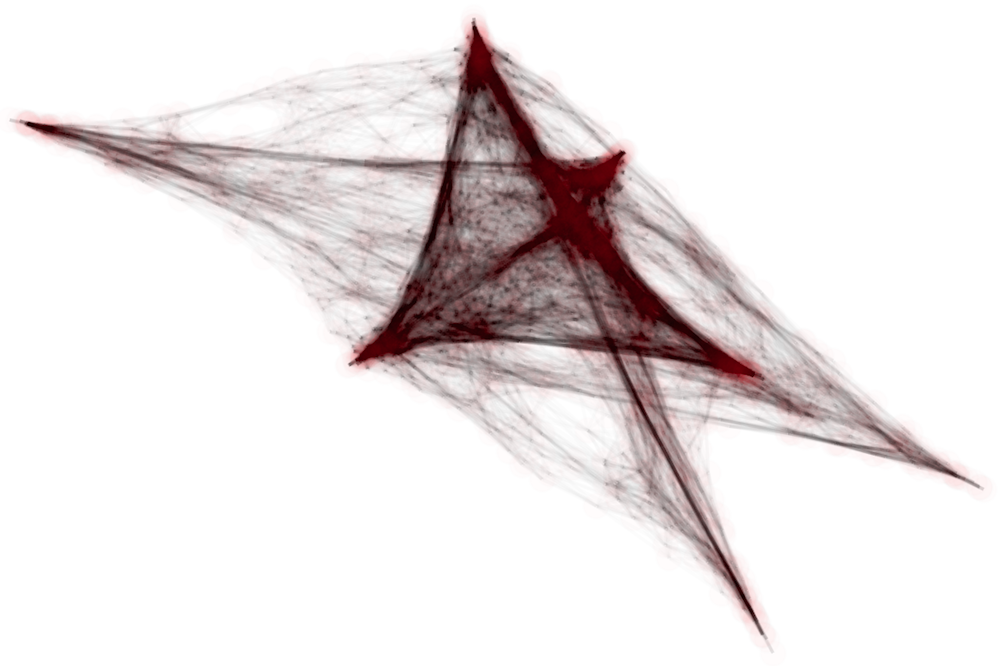
\includegraphics[height=2.5in]{figures/synthetic_graph_layout.png}
    \caption{A force directed layout was used on the graph.}
    \end{subfigure}
   
    \begin{subfigure}{\linewidth}
    \centering
    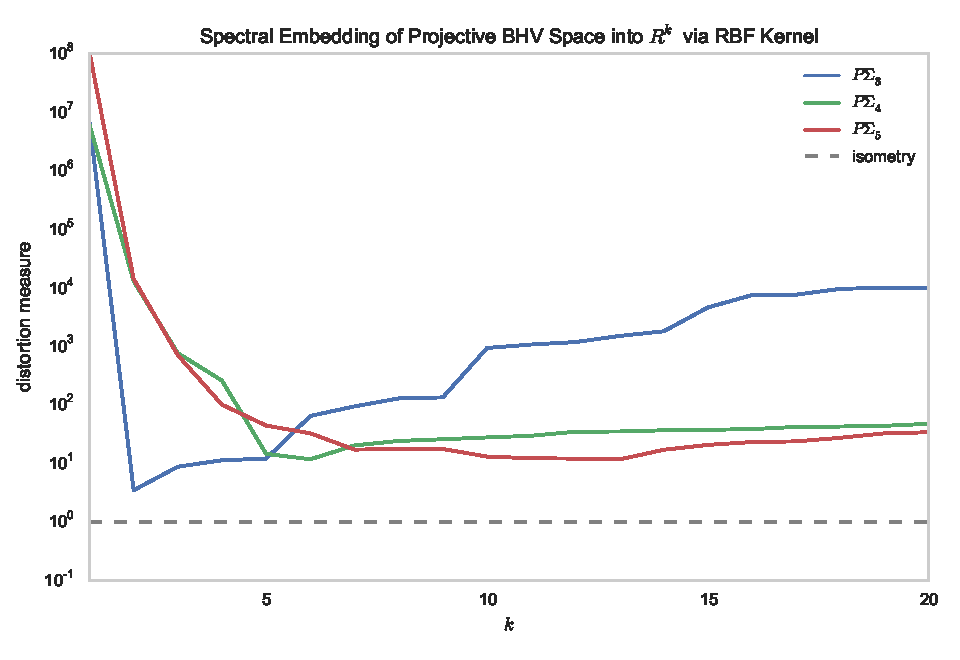
\includegraphics[height=2.5in]{figures/synthetic_distortion.pdf}
    \caption{Distortions of embedding the projective space into $\mathbb{R}^k$.}
    \end{subfigure}

    \caption{Computational implementation of $\mathbb{P}\Sigma_m$.}
     \label{fig:discretization}
\end{figure}

\subsection{Model selection}

We created three synthetic data sets upon which to demonstrate that plotting the DB-index for the k--Means implementation correctly discerns the optimal number of clusters present in the data.
The figures that have already been generated used the BHV distance metric, and need to be updated using the projective distance.

\begin{figure}[t!]
    \centering
    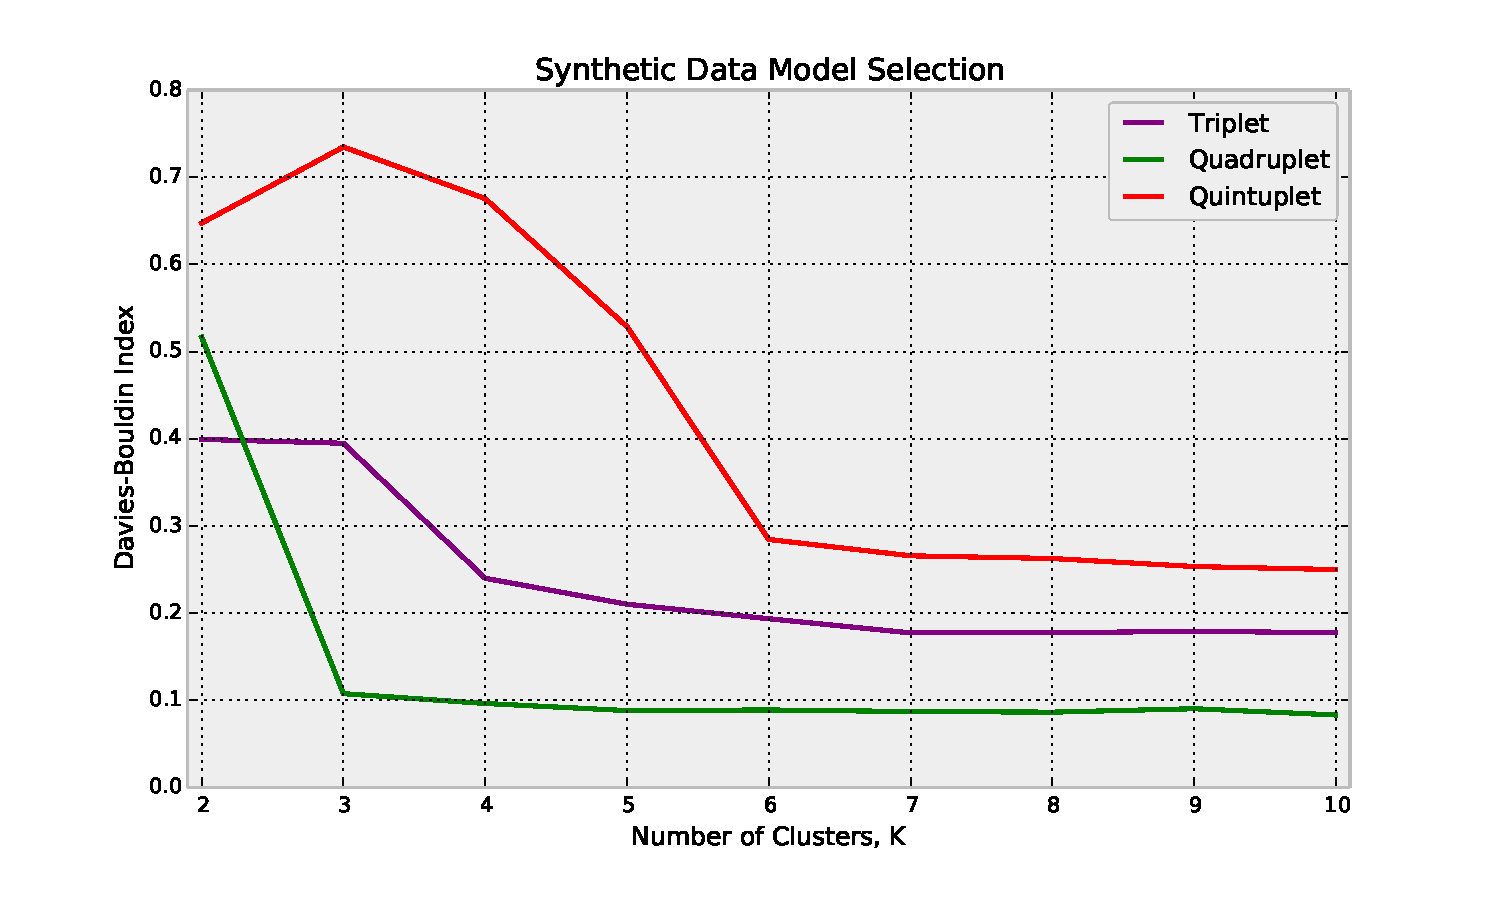
\includegraphics[height=3in]{figures/synthetic_davies_bouldin.pdf}
    \caption{We recover the correct value of K for clustering in different dimensions of projective space.}
    \label{fig:davies_bouldin}
\end{figure}


We also illustrate the order--1 Voronoi partition on the data, even though the optimal value of k is not 1.
We can mention the computational difficulty with computing the order--k Voronoi partition or we could man up and figure out how to actually do it.
The tesselation suggests a ``prognostic landscape in the space of tumor evolutionary modes.'' 


%\subsection{Simulating stochastic processes}
%Here we implemented certain archetypes of tumor evolution as forward time simulations, and we observed the distributions they generated in the EMS.
%Here we also examined diffusive processes in $\Sigma_m$ to gain intuition about exponential family distributions.

%%%%%%%%%%%%%%%%%%%%%%%%%%%%%%%%%%%%%%%%%%%%%%%%%%%%%%%%%%%%%%%%%%%%%%%%%%%%%%%%%%%%%%%%%%%%%%%%%%%%
%%%%%%%%%%%%%%%%%%%%%%%%%%%%%%%%%%%%%%%%%%%%%%%%%%%%%%%%%%%%%%%%%%%%%%%%%%%%%%%%%%%%%%%%%%%%%%%%%%%%

\section{Assessing predictive value of genomic information in cancer genomic data}\label{sec:cancer}

Clinical progression of cancer is believed to be intimately related to the accumulation of genomic alterations in tumor cells.
A small subset of protein coding genes have been implicated in the pathogenesis of certain cancer types, either as activated oncogenes or inactived tumor suppressors.
Documenting the mutational status of the protein coding genome at diagnosis via whole exome sequencing (WES) or even whole genome sequencing (WGS) is increasingly becoming a standard of care at university hospitals.
Targeted small-molecule inhibitors may be available for patients with mutations yielding constitutively active oncogenic proteins, or, as can be the case, a mutation in a signaling pathway can disqualify a patient from receiving pharmacologic blockade of the pathway upstream.
\textit{KRAS} (intracellular) mutations, for example, are known to negate the efficacy of EGFR blockade, which acts at the cell membrane.
A key question, however, is whether the mutational spectrum observed at diagnosis will be representative of the tumor throughout the disease course, and to what extent mutations will be gained or lost with treatment.

A tumor is a dynamic and heterogeneous compartment, and it is not clear yet what the hallmarks of tumor evolution are over the full disease course.
Longitudinal sequencing of tumor series provide the best data for studying the evolutionary patterns of cancer \cite{wang2015tumor} and to find early markers of progression \cite{rossi2014clinical}.
Such efforts are sure to accelerate with the widespread adoption of genomic techniques in clinical medicine.
WES is typically performed at a sufficient depth of coverage to characterize the genotype of the dominant cell fraction, termed the dominant clone.
At this level of resolution one can characterize the evolution via the degree of branching observed in the dominant clone.
Chemotherapy represents a powerful selective pressure on the tumor, and it is of interest to calculate the proportion of mutations observed at diagnosis that persist at a later clinical time point.
Two published studies, in chronic lymphocytic leukemia and relapsed glioma, show a clear effect of chemotherapy on the evolution of the dominant clone.

\subsection{Disruption of linear evolution by therapy in chronic leukemias}

Chronic lymphocytic leukemia (CLL) is the most common leukemia in adults, primarily affecting the elderly population (median age at diagnosis is 70).~\cite{smith2011incidence}
CLL was classically considered a very indolent disease, with patients often dying of causes unrelated to the cancer, however it is increasingly being appreciated that the prognosis of CLL is highly variable.
CLL is a proliferative disorder of B-lymphoctyes characterized by a steady accumulation of clonal, non-functional B-cells.
Treatment strategies vary greatly given the heterogeneity in disease course, ranging from watchful waiting, to localized radiation, to systemic chemotherapy.
None of these approaches are considered potentially curative; the only such option is bone marrow transplant.

The fact that CLL is a relatively indolent malignancy allows a longer time window than usual for studying clonal evolution.
A recent genomic study~\cite{landau2013evolution} performed WES on 160 CLL cases covering the spectrum of clinical courses the disease can take.
This data established a space of recurrent alterations, which was then used to genotype 18 patients for whom two time points were available.
Of these 18 patients, 10 of 12 treated with chemotherapy underwent clonal evolution compared to only 1 of 6 receiving no treatment according to the authors of the study.
We combine the 18 patients of \cite{landau2013evolution} with those of a similar study~\cite{schuh2012monitoring} wherein 3 CLL patients received chemotherapy and were sequenced at multiple time points.
The multiple time points for the 3 patients studied in~\cite{schuh2012monitoring} are decomposed into all combinatorial triplets.
Therefore, there are a total of 18 phylogenetic trees inferred from \cite{landau2013evolution} and 12 phylogenetic trees inferred from \cite{schuh2012monitoring}.
In Figure N, we map this data to $\mathbb{P}\Sigma_3$ and color based on treatment status.

\begin{figure}
    \begin{subfigure}{0.5\linewidth}
    \centering
    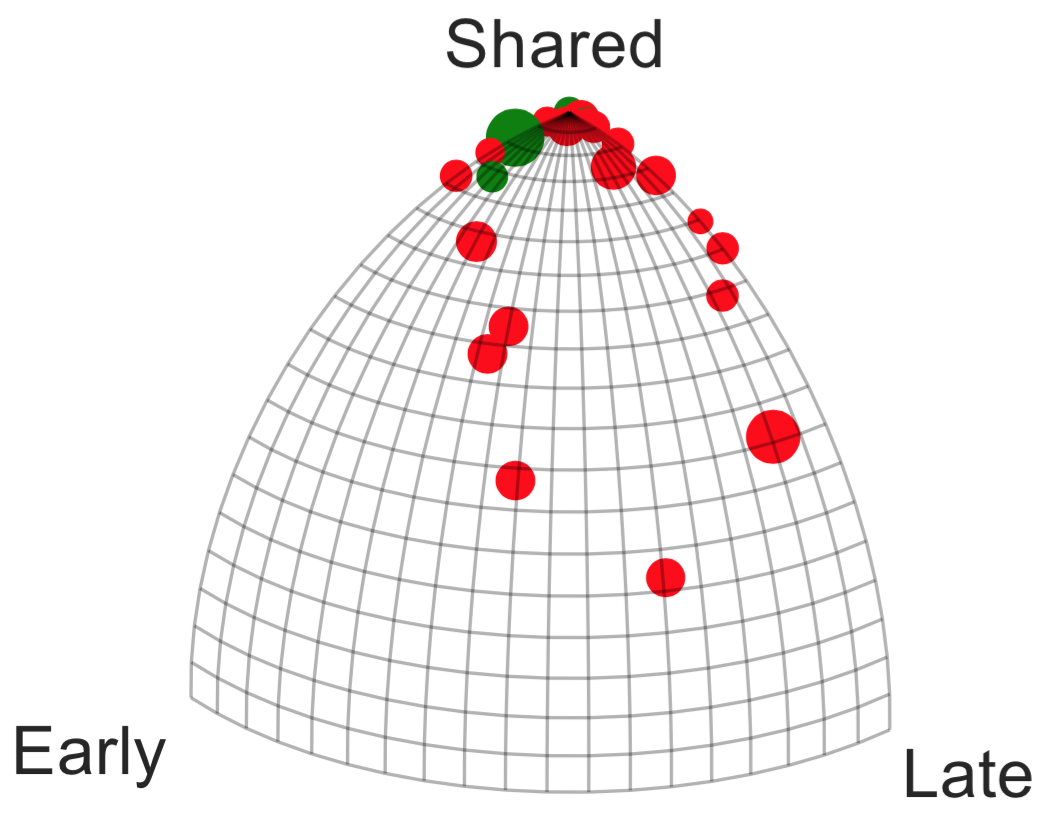
\includegraphics[height=2.2in]{figures/CLL_triplet.png}
    \caption{caption goes here.}
    \end{subfigure}
    ~
    \begin{subfigure}{0.5\linewidth}
    \centering
    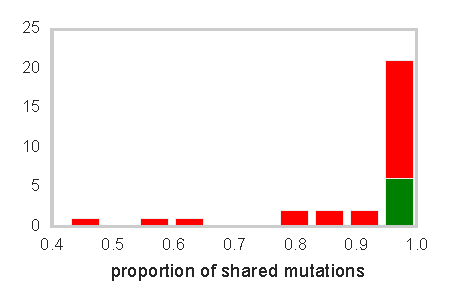
\includegraphics[height=2in]{figures/CLL_histogram.pdf}
    \caption{caption goes here.}
    \end{subfigure}

    \caption{Frozen vs. Branched evolution observed in CLL patients receiving no chemotherapy and chemotherapy respectively. Cases with no chemotherapy are represented in red while cases involving chemotherapy are represented in green. Colored circles are scaled by patients' total number of mutations. The centroids of the two distributions are represented as gold stars, and their associated phylogenetic trees are visualized.}
    \label{fig:chemoCLL}
\end{figure}

From a clinical standpoint, the central question is whether treatment promotes evolution of the cancer and whether there is strong evidence for avoiding cytotoxic therapy in patient management.
Quite clearly the distribution of 6 untreated patients resembles a frozen pattern, while the 15 patients who underwent chemotherapy have a far more branched mode of evolution.
The 95\% CI for the distance between the centroids of the treated / untreated groups is (0.15, 0.36), under 1000-fold bootstrap resampling.
The analogous intervals for untreated / untreated and treated / treated are (0.01, 0.14) and (0.02, 0.16) respectively.
The centroids of these clinically distinct sets of patients are statistically well-resolved.

\subsection{The geometry of a tree is associated with grade at relapse in gliomas}

Low grade gliomas (LGG) are a set of tumors of the central nervous system most often involving astrocytes or oligodendrocytes.
They are distinguised from high grade gliomas (III, IV), such as glioblastoma multiforme, by the absence of anaplasia and have a more favorable prognosis.
Surgery alone is not considered curative for LGG and patients are typically treated with adjuvant radiation therary, chemotherapy, or both.
If a patient relapses, the tumor may be observed to have a higher grade at that time.
Johnson \textit{et al.} studied a cohort of 23 LGG patients who relapsed, many of whom were treated with the chemotherapeutic agent temozolamide (TMZ).~\cite{johnson2014mutational}
WES was performed on tumor tissue at diagnosis and at relapse in an effort to characterize the evolution of recurrent glioma.

\begin{figure}
    \begin{subfigure}{0.5\linewidth}
    \centering
    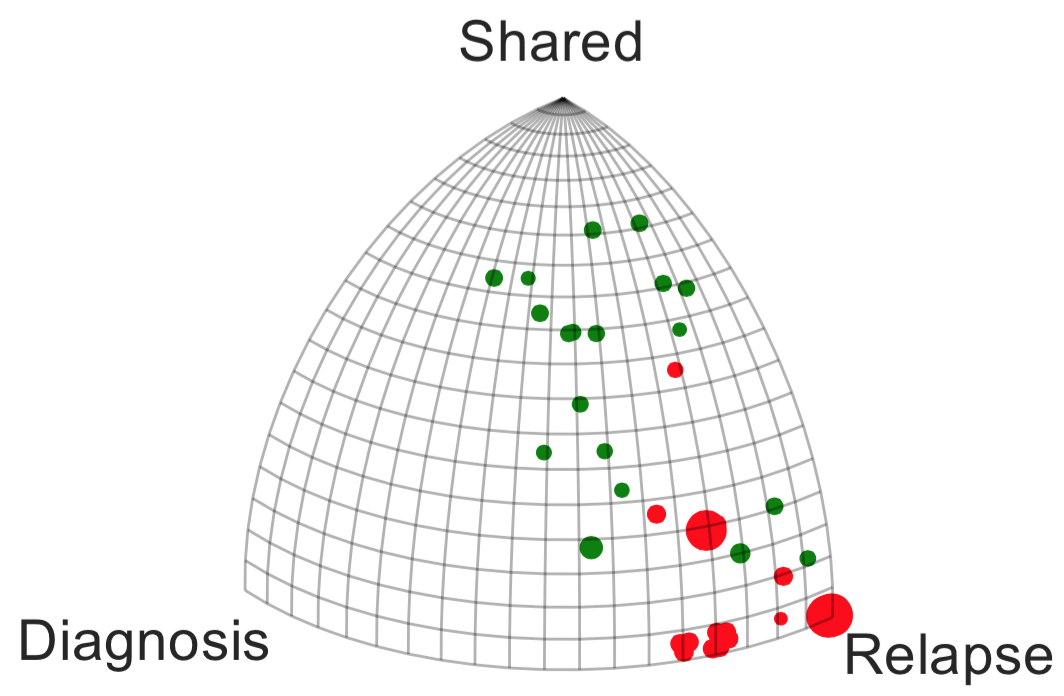
\includegraphics[height=2.2in]{figures/glioma_triplet.png}
    \caption{caption goes here.}
    \end{subfigure}
    ~
    \begin{subfigure}{0.5\linewidth}
    \centering
    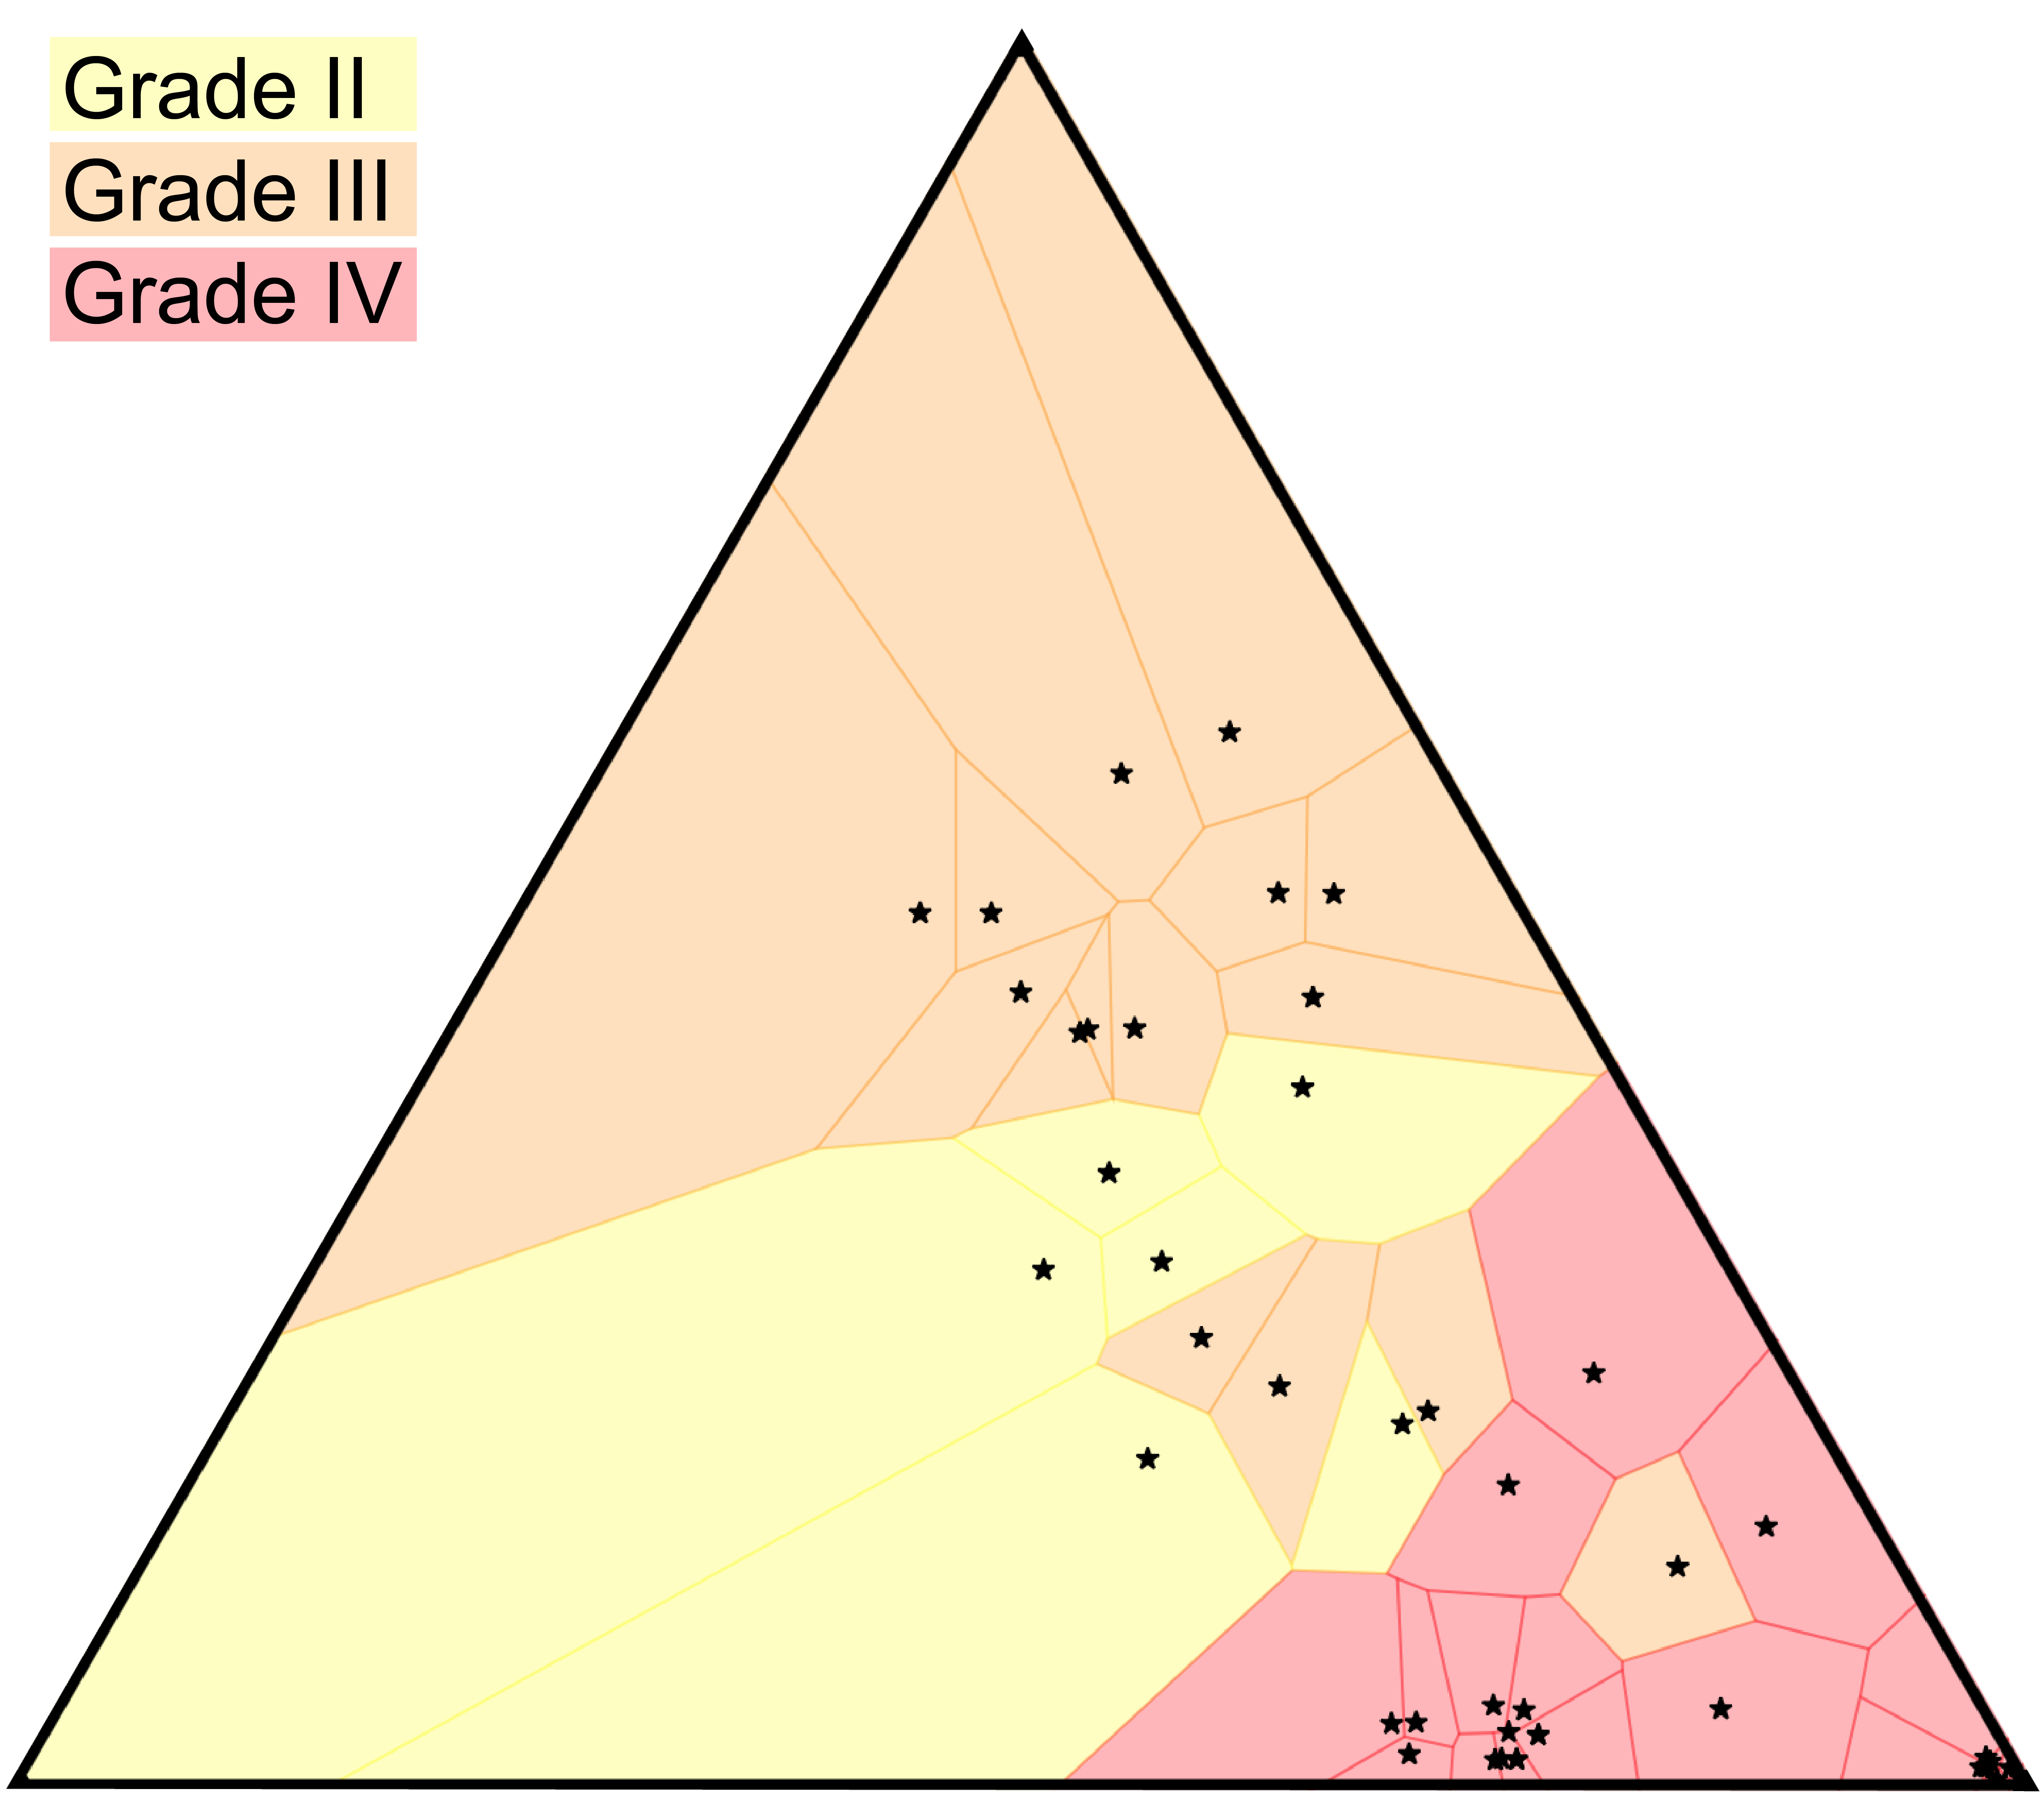
\includegraphics[height=2in]{figures/glioma_voronoi_stage.png}
    \caption{caption goes here.}
    \end{subfigure}

    \caption{Evolution of recurrent glioma.}
    \label{fig:gliomaTMZ}
\end{figure}

TMZ is an alkylating agent that directly damages the cellular genome, and accordingly we see that the subset of patients that were treated with TMZ show a greater acquisition of relapse-specific mutations.
The 95\% CI for the distance between the centroids of the treated / untreated groups is (0.31, 0.48), under 1000-fold bootstrap resampling.
The analogous intervals for untreated / untreated and treated / treated are (0.02, 0.13) and (0.02, 0.16) respectively.
TMZ treatment status defines two statistically well-resolved sub-populations of patients with respect to the shape of their evolutionary behavior.
Also of interest is the apparent correlation between the geometry of the phylogenetic tree and the histologic grade at relapse.
A 1-nearest neighbor classifier of this trinary observable (grade II, III, or IV at relapse) yields 85\% accuracy under two-fold CV, and the accuracy does not improve with larger values of $k$.
The tesselation of the space associated to a 1-nearest neighbor classifier is known as a Voronoi diagram, and we have colored the cells in accordance with the grade at relapse.

%%%%%%%%%%%%%%%%%%%%%%%%%%%%%%%%%%%%%%%%%%%%%%%%%%%%%%%%%%%%%%%%%%%%%%%%%%%%%%%%%%%%%%%%%%%%%%%%%%%%
%%%%%%%%%%%%%%%%%%%%%%%%%%%%%%%%%%%%%%%%%%%%%%%%%%%%%%%%%%%%%%%%%%%%%%%%%%%%%%%%%%%%%%%%%%%%%%%%%%%%

\section{Phylogenetic dimensional reduction}\label{sec:flu}

Phylogenetic trees are often too complex to visualize and analyze; however, lower dimensional representations (such as ``tree'' dimensionality reduction procedures) are able to capture important phenomena. 

\begin{figure}
    \begin{subfigure}{\linewidth}
    \centering
    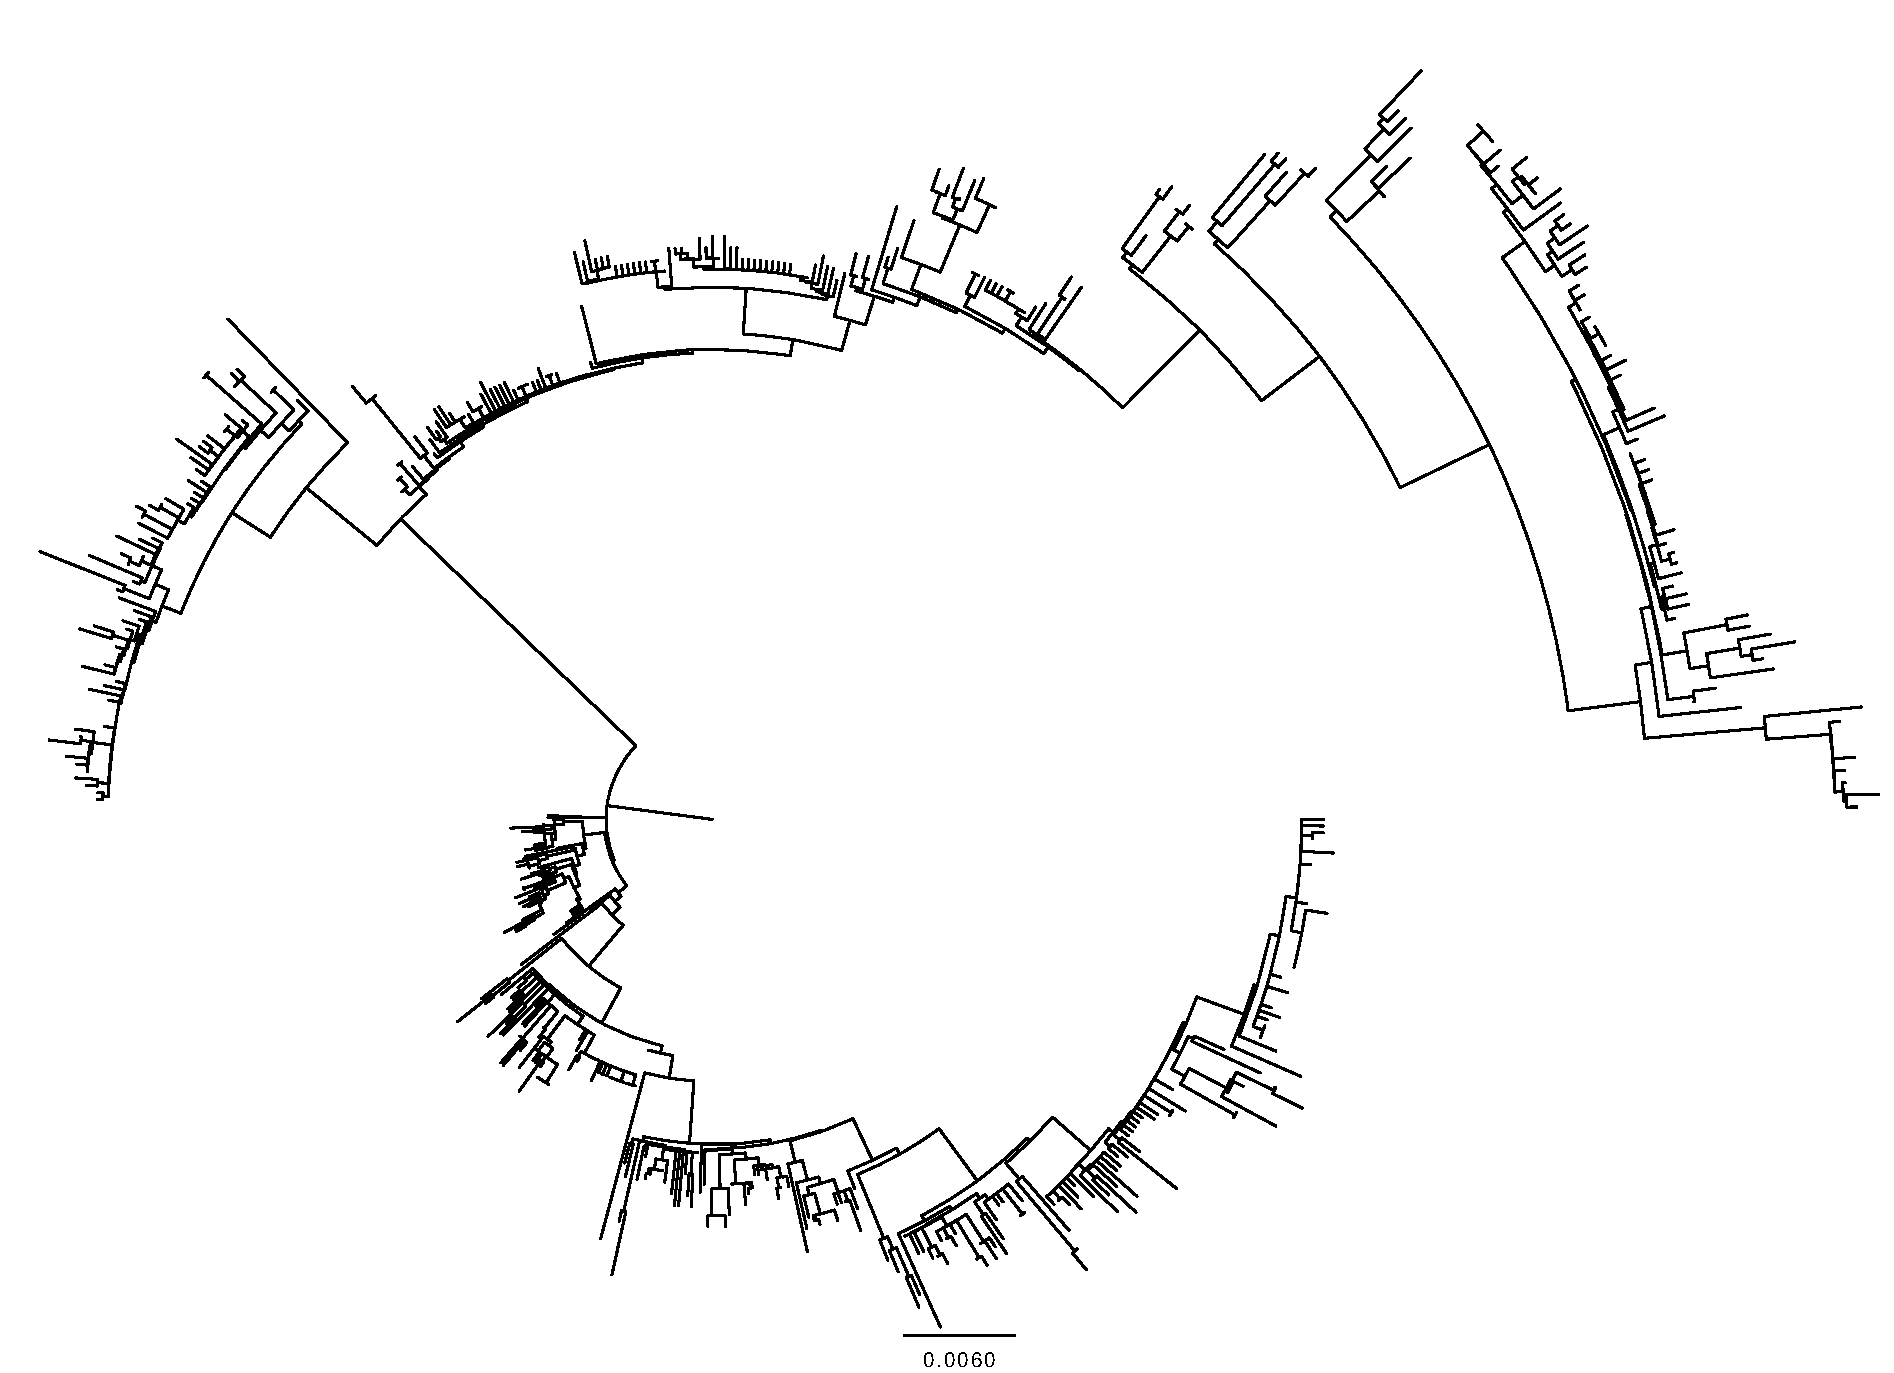
\includegraphics[width=4in]{figures/LargeFluTree-NYH3N2-NJ.pdf}
    \caption{Large tree.}
    \end{subfigure}

    \begin{subfigure}{\linewidth}
    \centering
    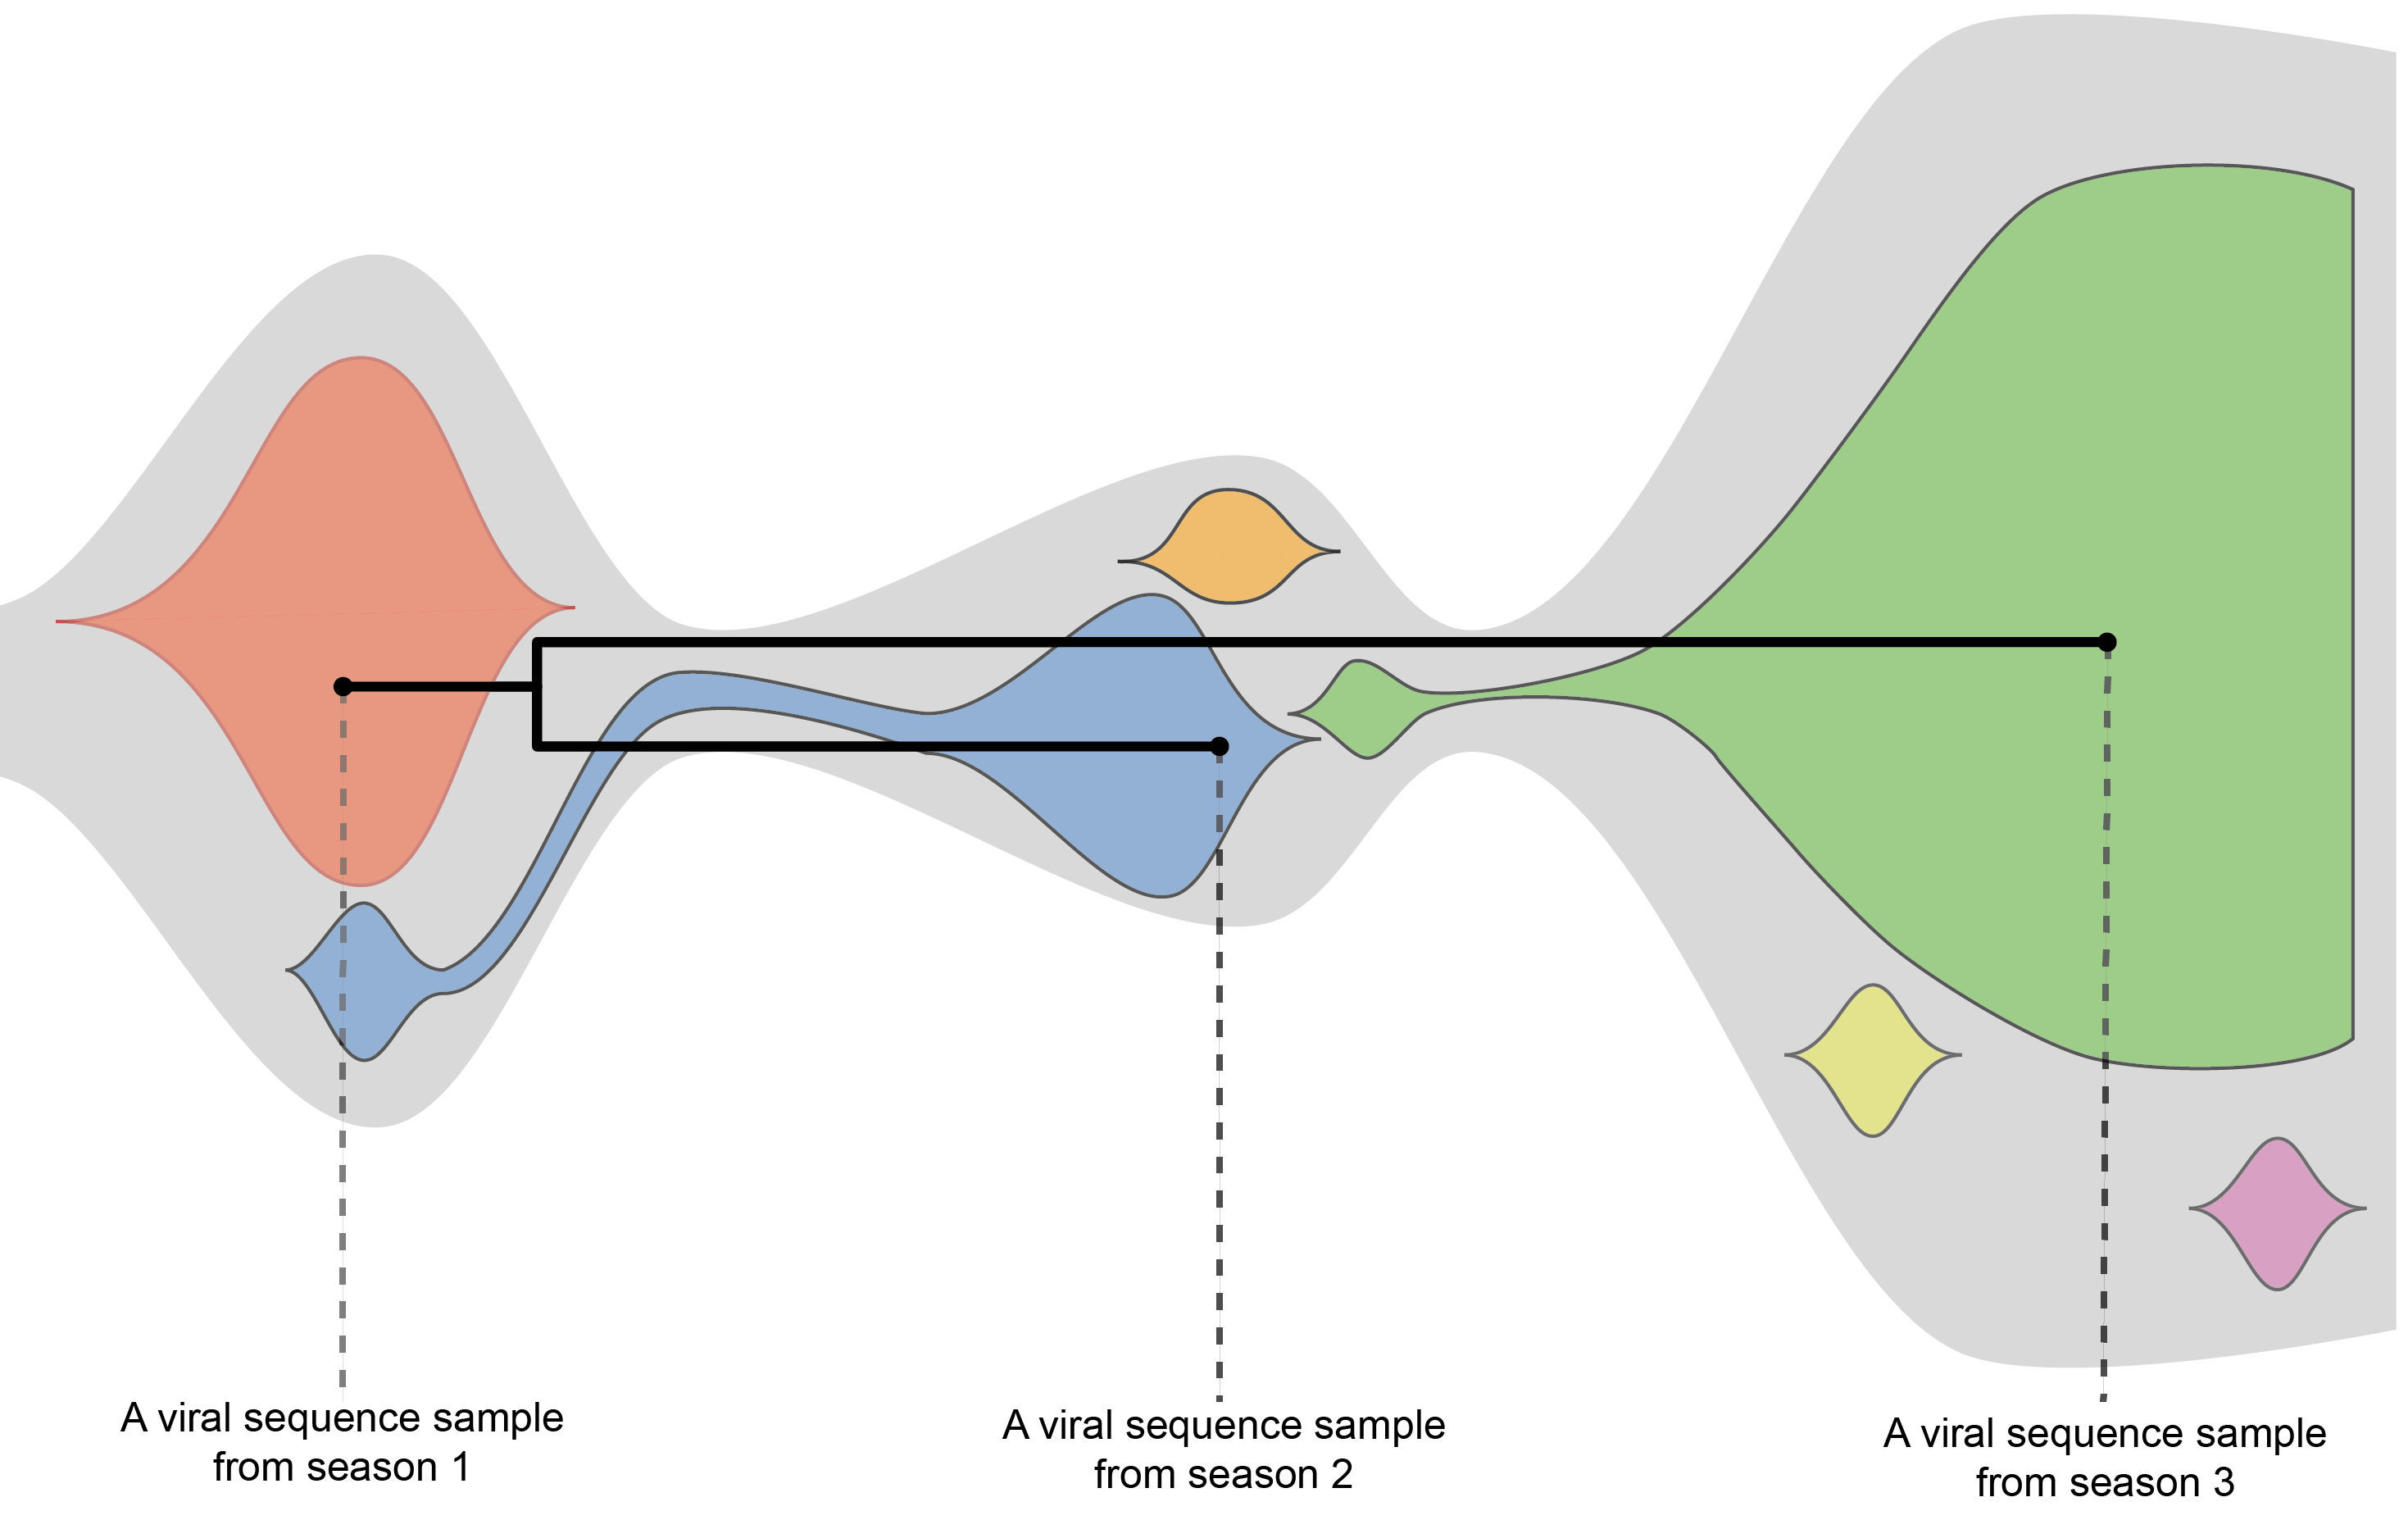
\includegraphics[width=4in]{figures/influenza_schematic_part1.png}
    \caption{Scheme.}
    \end{subfigure}
   
    \begin{subfigure}{\linewidth}
    \centering
    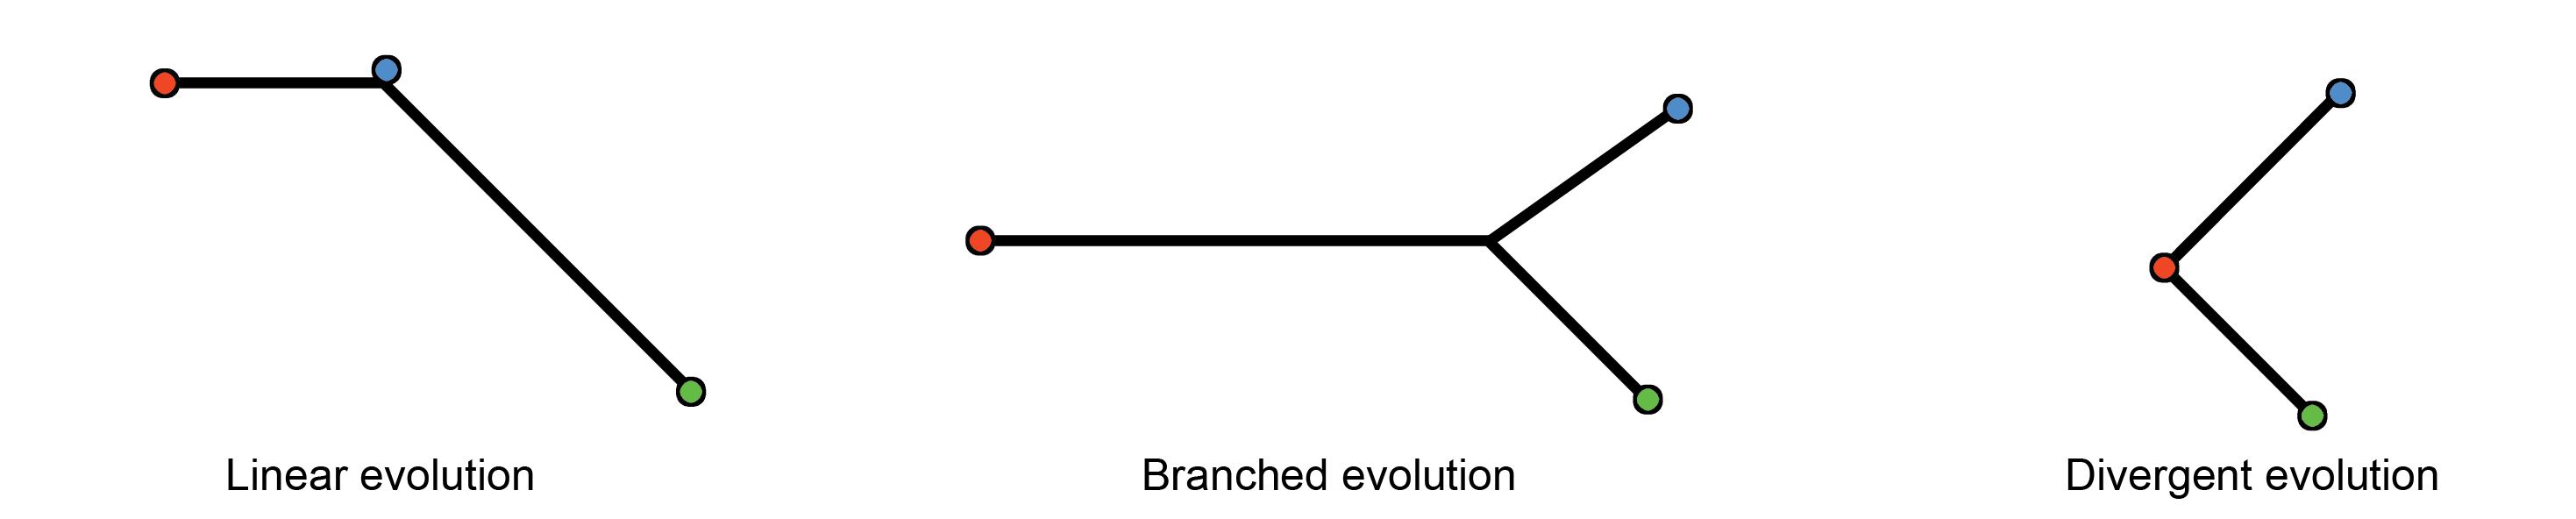
\includegraphics[width=4in]{figures/influenza_schematic_part2.png}
    \caption{Small tress.}
    \end{subfigure}

    \caption{Evolution of influenza A virus presenting clear seasonal variation.(a) Identifying statistical patterns in large trees is often difficult. This phylogenetic tree of the hemmagglutinin (HA) segment from 580 H3N2 influenza viruses across 15 seasons  can be  sub-sampled for statistical analysis in lower dimensional projections. (b)  Due to genomic drift, new strains appear each season, dominating the periods of viral expansion. (c) Different clones across seasons can be characterized through sub-sampling viral populations. If the pattern is highly linear, clones at some season will be directly related to emerging clones in the following seasons. However, if clones emerge that are genetically very different from previously sampled clones (on the right, branched or divergent behaviors) it will be difficult to make predictions based on recent samples. Currently influenza vaccine depends critically on these data and these predictions.}
     \label{fig:flu_schematic}
\end{figure}

The approach we present here is based on sub-sampling of a larger structure and preforming statistical analysis in lower dimensional projections.
This procedure has two advantages in relation to larger trees: on the one hand one can easily visualize, extract, perform statistical analysis, and interpret different types of evolutionary relationships.
On the other hand, it avoids the problem of scalability of phylogenetic algorithms with the number of leaves.
One particular application of these projections is the identification of clonal replacement, when a clone, not directly descending from the dominant clone at the previous phase, shows dominant presence \ref{fig:flu_schematic}.
The reason for this clonal replacement phenomena could be manifold, from strong bottlenecks associated to ancestral clone's loss of fitness or a sub-clone's rapid adaptation.
Here, we present the analysis of two distinct datasets.
We first study the evolution of influenza A virus in humans and show the presence of clonal replacement events that lead to vaccine failure.
Then, we investigate clonal evolution in patient-derived xenografts at single-cell levels and characterize tumor evolutionary trajectories.

\subsection{Detecting new dominant strains in seasonal influenza}

The design of influenza vaccine is based on samples of previous years under the assumption that virus in the coming season will be antigenically similar to most recent circulating strains. This is an strong assumption, as relatively small genetic changes in the genome of the virus can cause drastic antigenic shif.  Influenza vaccine failures are usually associated with the emergence of new clones with novel antigenic properties that have replaced recent circulating strains. Here we study how the emergence of a novel subclone could be identified by the unusual/unexpected tree structures. For this purpose we study the recent history of influenza A H3N2 using 580 sequences of hemmagglutinin (HA) collected in New York State between 1993 and 2007.


The influenza virus genome consists of eight single-stranded RNA segments, two of which code the antigenic surface glycoproteins, hemagglutinin (HA) and neuraminidase (NA).
The evolution of influenza viruses follows two distinct patterns: 1) genomic drift, the random accumulation of mutations due to antigenic pressure and high error rate in the replication process; 2) reassortment, the mixing of segments from two different strains during co-infection.
The former is the reason behind annual updates of the influenza vaccine; the latter, when introducing viral segments from non-human reservoirs, has led to major pandemics over the past century~\cite{rabadan2007evolution, rabadan2008non} and  was particularly associated with the emergence of the 2009 H1N1 pandemic.~\cite{trifonov2009geographic, solovyov2009cluster}
In 1968, the reassortment of then-circulating H2N2 with avian strains created H3N2 viruses, which have since been infecting human population.
Reassortment of seasonal strains can also contribute to vaccine failure as low frequency hemagglutinin segments can combine with highly transmissible strains. In particular, reassortment of two H3N2 clades during the 2002-2003 season resulted in a major epidemic and higher incidents of vaccine failure in the succeeding season.~\cite{centers2004preliminary}

\begin{figure}
    \centering
    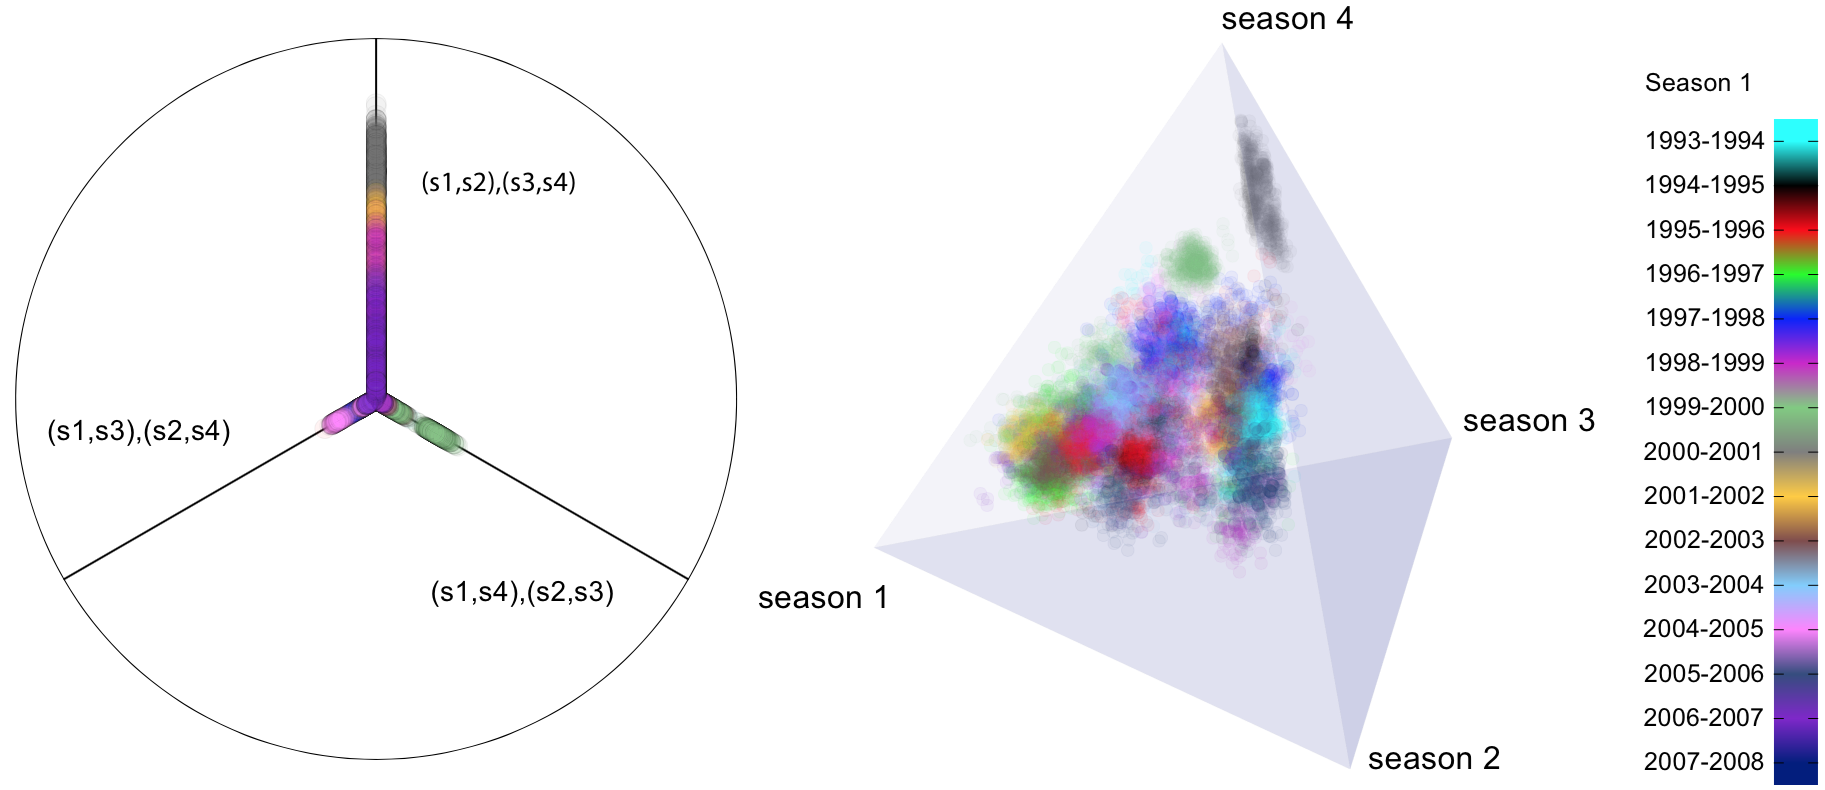
\includegraphics[width=6in]{figures/influenza_quad.png}
    \caption{Superimposed $\mathbb{P}\Sigma_4$ spaces relating four consecutive influenza seasons, using 580 influenza A H3N2 strains collected from New York from 1993 to 2009.}
    \label{fig:flu_quad}
\end{figure} 

Using 580 H3N2 strains collected in New York State between 1993 and 2009, we relate HA sequences from one season to those from the succeeding ones.
We pick random strains from four and five consecutive seasons, and using neighbor-joining based on hamming distances, generate un-rooted trees compromising 14 $\mathbb{P}\Sigma_4$ (Fig \ref{fig:flu_quad}) and 13 $\mathbb{P}\Sigma_5$  (Fig \ref{fig:flu_quint}) spaces.
The majority of spaces for HA show linear evolution of influenza from one season to another, indicating genetic drift as virus's dominant evolutionary process.
We, however, detect distinct clusters of trees in HA'„s evolutionary spaces that indicate clonal replacement and reemergence of strains in the 2002-2003 season genetically similar to those circulating in the 1999-2000 season. [NEED STATISTICS]
These results corroborate previously published whole-genome and segment-specific phylogenetic analyses.~\cite{holmes2005whole}

\begin{figure}
    \centering
    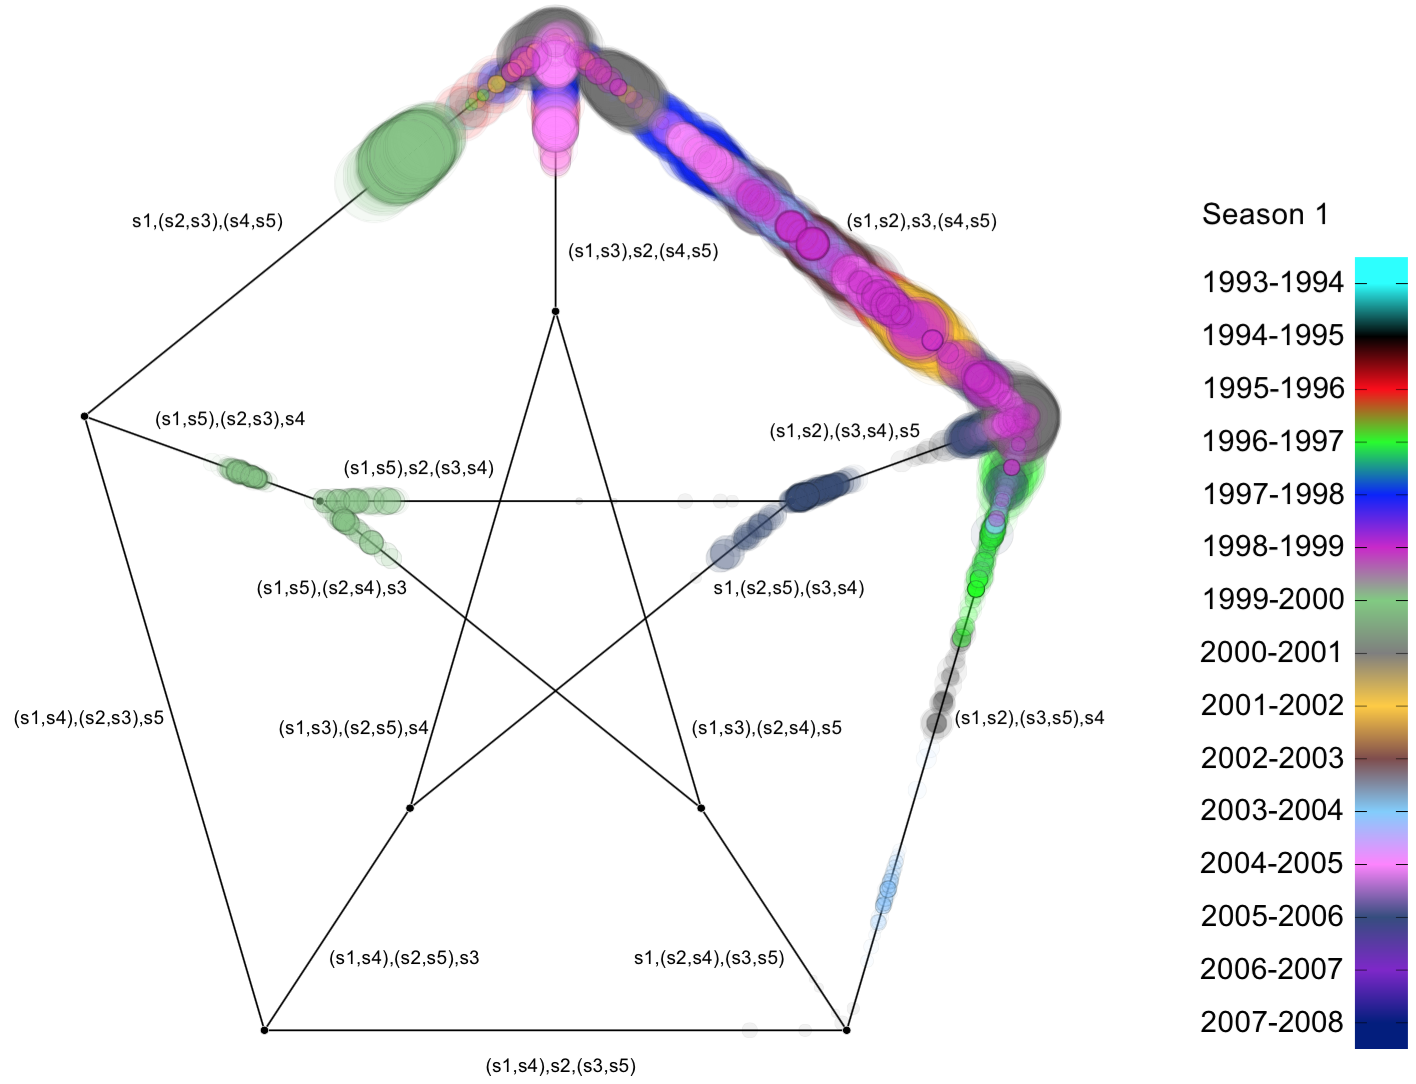
\includegraphics[width=6in]{figures/influenza_quint.png}
    \caption{Superimposed $\mathbb{P}\Sigma_5$ spaces relating five consecutive influenza seasons, using 580 influenza A H3N2 strains collected from New York from 1993 to 2009.}
    \label{fig:flu_quint}
\end{figure} 

\subsection{Clonal heterogeneity from single cell tumor genomics}

The recent development of single cell transcriptomics and genomics is providing an opportunity to study the role of clonal heterogeneity in tumors~\cite{navin2011tumour, eirew2014dynamics, patel2014single} and to identify small, previously uncharacterized cell populations~\cite{grun2015single}.
Single cell data provides the opportunity to sample complex populations by studying the dynamics of different cell subpopulations.
However, these data create new challenges associated with a large number of cells necessitating comprehensive sampling of the process. 

Patient-derived xenografts, generated by transplanting tumor tissue into immunodeficient mice, have also emerged as reliable models for studying tumor evolutionary dynamics and heterogeneity.
Here, we use breast cancer single-nucleus deep-sequence data obtained from three engrafting passages~\cite{eirew2014dynamics}, compromising 55 segregating sites.
These sites include variants that Eirew \textit{et al.} associated with eight distinct clonal clusters using bulk DNA.

\begin{figure}
    \centering
    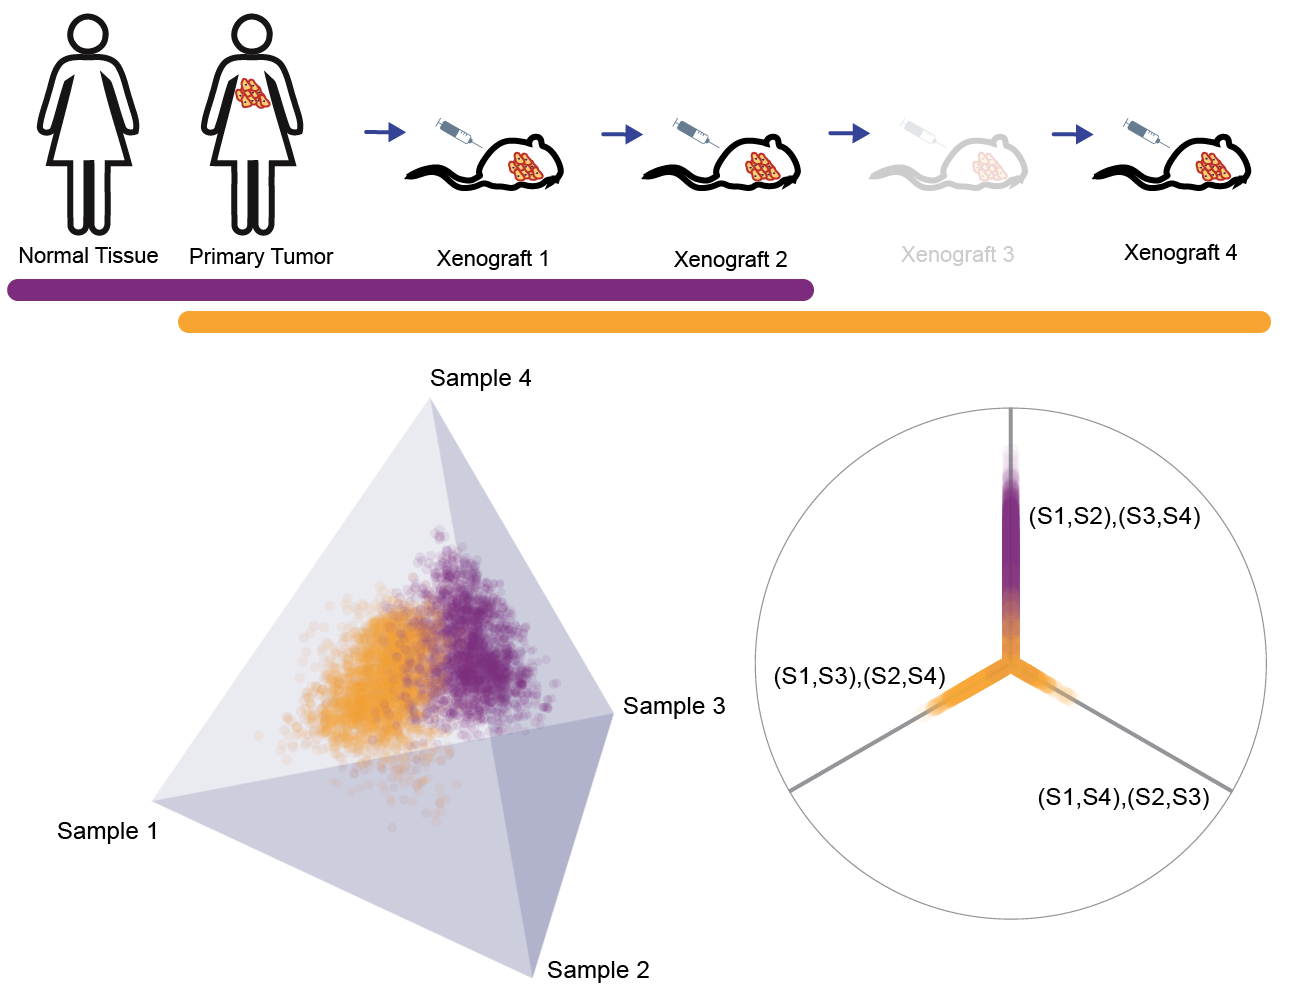
\includegraphics[height=4in]{figures/xenograft_single_cell.png}
    \caption{Single cell analysis of tumor evolution in a breast cancer derived xenograft model. Single-nucleus deep-sequence data obtained from passage 1, 2, and 4. Single-cell data from primary tumor is not available, however  Eirew \textit{et al.}~\cite{eirew2014dynamics} identified eight distinct clusters. These data were used to generate two $\mathbb{P}\Sigma_4 $ spaces.}
    \label{fig:xenograft}
\end{figure} 

Single-cell data from the primary tumor is not available, however we generate eight cluster-representative sequences and using 27, 36, and 27 single nuclei from the first, second, and fourth passage, we sub-sample 3,000 trees from all possibilities and project the data into $\mathbb{P}\Sigma_4 $.
First, we include trees relating the germ-line sequence, a randomly selected cluster-representative sequence form the primary tumor, and randomly selected single-nucleus sequences from the initial two xenograft passages.
Then, in a second analysis, we include trees relating a randomly selected cluster-representative sequence form the primary tumor and randomly selected single-nucleus sequences from three consecutive xenograft passages.
Our results (Fig \ref{fig:xenograft}) show consistent linear evolution from primary tumor towards xenograft samples.
However, we observe significant divergence of tumor clones during multiple engraftments. [NEED STATISTICS: standard deviation in each space; clustering too, 1st one should be 1 cluster, 2nd one 3 clusters. etc.]

%%%%%%%%%%%%%%%%%%%%%%%%%%%%%%%%%%%%%%%%%%%%%%%%%%%%%%%%%%%%%%%%%%%%%%%%%%%%%%%%%%%%%%%%%%%%%%%%%%%%
%%%%%%%%%%%%%%%%%%%%%%%%%%%%%%%%%%%%%%%%%%%%%%%%%%%%%%%%%%%%%%%%%%%%%%%%%%%%%%%%%%%%%%%%%%%%%%%%%%%%

\section{Conclusions}\label{sec:conclusions}

There is an exciting frontier of open questions related to evolutionary moduli spaces.
One obvious question is how our visualization framework can scale to much larger numbers of sequential tissue samples.
In the limit of extremely dense sampling of a patient's tumor progression, our current strategy may become unwieldy due to the high dimensionality of the spaces.
Even for the case of 6 samples it is challenging construct a succinct visualization of $\mathbb{P}\Sigma_6$, a space in which each patient could be represented by a point.
An alternate strategy is to use a sliding window to decompose densely sampled patients into overlapping tuples of length $3 \leq j \leq 5$.
Over the course of a densely sampled tumor progression one could thus observe the local evolutionary relationships between adjacent samples.
A patient with $m$ tissue samples would then be decomposed into $m - j$ tuples, each of which correspond to a point in $\mathbb{P}\Sigma_j$, thus tracing out a curve in the projective space.
The underlying biology of the cancer would be encoded by the shape, direction, and neighborhood of confinement of the curve on $\mathbb{P}\Sigma_j$.
This approach to visualization scales nicely with $m$, since there would be more tuples with which to fit a curve, but replaces point clouds with sets of curves as the representational scheme for a patient population.

Another question that looms large is how to define useful probability distributions, such as those of the exponential family, on $\Sigma_m$.
The k--means algorithm demonstrated earlier, for example, can be thought of as a limiting case of hard assignment in a mixture of $k$ Gaussian densities.
Any attempt at soft assignment of patients to an underlying probabilistic clustering model would necessarily rely upon well defined notions of distributions in $\Sigma_m$.
Defining distributions on $\Sigma_m$ would open a more direct communication between evolutionary moduli spaces and the field of generative modeling.
One potentially fruitful approach for approximating probability densities such as the normal distribution is to simulate diffusive processes in $\Sigma_m$, taking advantage of the relationship between random walks and their limiting distributions.

%%%%%%%%%%%%%%%%%%%%%%%%%%%%%%%%%%%%%%%%%%%%%%%%%%%%%%%%%%%%%%%%%%%%%%%%%%%%%%%%%%%%%%%%%%%%%%%%%%%%
%%%%%%%%%%%%%%%%%%%%%%%%%%%%%%%%%%%%%%%%%%%%%%%%%%%%%%%%%%%%%%%%%%%%%%%%%%%%%%%%%%%%%%%%%%%%%%%%%%%%

\subsection*{Acknowledgments}

The authors gratefully acknowledge the constructive feedback of Daniel Rosenbloom.
This work is supported by a TL1 personalized medicine fellowship (5TL1TR000082), and NIH grants (R01 CA179044, R01CA185486, R01GM117591, U54 CA193313).

%%%%%%%%%%%%%%%%%%%%%%%%%%%%%%%%%%%%%%%%%%%%%%%%%%%%%%%%%%%%%%%%%%%%%%%%%%%%%%%%%%%%%%%%%%%%%%%%%%%%
%%%%%%%%%%%%%%%%%%%%%%%%%%%%%%%%%%%%%%%%%%%%%%%%%%%%%%%%%%%%%%%%%%%%%%%%%%%%%%%%%%%%%%%%%%%%%%%%%%%%

\bibliography{refs}

\end{document}
